% !TEX TS-program = pdflatex
% !TEX encoding = UTF-8 Unicode

% This is a simple template for a LaTeX document using the "article" class.
% See "book", "report", "letter" for other types of document.

\documentclass[11pt]{article} % use larger type; default would be 10pt

\usepackage[utf8]{inputenc} % set input encoding (not needed with XeLaTeX)

%%% Examples of Article customizations
% These packages are optional, depending whether you want the features they provide.
% See the LaTeX Companion or other references for full information.

%%% PAGE DIMENSIONS
\usepackage{geometry} % to change the page dimensions
\geometry{a4paper} % or letterpaper (US) or a5paper or....
\geometry{margin=1in} % for example, change the margins to 2 inches all round
% \geometry{landscape} % set up the page for landscape
%   read geometry.pdf for detailed page layout information

\usepackage{graphicx} % support the \includegraphics command and options

\usepackage[parfill]{parskip} % Activate to begin paragraphs with an empty line rather than an indent
\setlength{\parindent}{1cm}

%%% PACKAGES
\usepackage{booktabs} % for much better looking tables
\usepackage{array} % for better arrays (eg matrices) in maths
\usepackage{paralist} % very flexible & customisable itemizes (eg. enumerate/itemize, etc.)
\usepackage{verbatim} % adds environment for commenting out blocks of text & for better verbatim
\usepackage{subfig} % make it possible to include more than one captioned figure/table in a single float
\usepackage{amssymb} % more 'unusual' symbols not included in standard LaTeX package
\usepackage{enumitem}
\usepackage{amsmath}
\usepackage{comment}
\usepackage{color}
\usepackage{graphicx}
\usepackage{subcaption}
\usepackage{xspace}
\usepackage{gensymb}
\usepackage[font=small,format=plain,labelfont=bf,textfont=normal,justification=justified,singlelinecheck=false]{caption}
\usepackage{calligra}
\DeclareMathAlphabet{\mathcalligra}{T1}{calligra}{m}{n} 
\DeclareFontShape{T1}{calligra}{m}{n}{<->s*[2.2]callig15}{} 
\usepackage{dcolumn}
\ldots
\newcolumntype{d}[1]{D{.}{\cdot}{#1} }
\newcommand{\centercell}[1]{\multicolumn{1}{C}{#1}}

% These packages are all incorporated in the memoir class to one degree or another...

%%% HEADERS & FOOTERS
\usepackage{fancyhdr} % This should be set AFTER setting up the page geometry
\pagestyle{fancy} % options: empty , plain , fancy
\renewcommand{\headrulewidth}{0pt} % customise the layout...
\lhead{}\chead{}\rhead{}
\lfoot{}\cfoot{\thepage}\rfoot{}


%%% SECTION TITLE APPEARANCE
\usepackage{sectsty}
\allsectionsfont{\sffamily\mdseries\upshape} % (See the fntguide.pdf for font help)
% (This matches ConTeXt defaults)

%%% ToC (table of contents) APPEARANCE
\usepackage[nottoc,notlof,notlot]{tocbibind} % Put the bibliography in the ToC
\usepackage[titles,subfigure]{tocloft} % Alter the style of the Table of Contents
\renewcommand{\cftsecfont}{\rmfamily\mdseries\upshape}
\renewcommand{\cftsecpagefont}{\rmfamily\mdseries\upshape} % No bold!

%%%Command Macros


%%% END Article customizations

\graphicspath{ {./images/} }

\title{The Mimas Leading Edge Anomaly: Thermal conductivity and grain cementation radius}
\author{M.J. Schaible, R.Johnson, L. Zhigilei}
%\date{} % Activate to display a given date or no date (if empty),
         % otherwise the current date is printed 

\begin{document}
\maketitle

\section{Abstract}

	Goals:
	\begin{itemize}
	\item Derive the thermal conductivity differences between inside/outside anomalous region on Mimas and Tethys
		\begin{itemize}
		\item Can the thermal conductivity differences be explained in terms of structural differences in the regolith?
		\item How does the thermal conductivity depend on grain contact: linearly or quadratically?
		\item Is Hertzian analysis sufficient to determine effective contact areas between grains?
		\end{itemize}
	\item Estimate effects of $>$1MeV electrons on grain cementation properties
		\begin{itemize}
		\item Determine energy deposition vs. depth profile of the electrons in the regolith from PENELOPE results.
		\item What is the heating effect on $\sim$50$\mu$m grains for each interaction?
		\item What are the relative thermal and near surface electronic excitation molecular desorption yields from pore surfaces?
			\begin{itemize}
			\item Use energy vs. depth to estimate grain heating for input into sintering equations. 
			\item Use thermal spike method to model electronic excitation desorption.
			\item How can Hayley simulations be used to help understand?
			\end{itemize}
		\item What is the gas production rate? How do gas readsorption time-scales compare to heat transfer time-scales?
		\item What are electron effects on crystal structure, esp. at the grain boundary? (comment)
		\item Using energy deposition profile and known W-value, estimate probability of excitations.
		\item Can the electron irradiation explain thermal conductivity differences?
		\end{itemize}
%	\item Estimate the proton defect creation, sintering, and gas production rates. Can they account for trailing hemisphere discolorations?
	\item Estimate time-scale for cementation increase to explain increased cementation
	\item Use published results to estimate gardening rate due to micrometeorite bombardment and compare to sintering time-scale.
	\end{itemize}

	Thermal models have been developed to simulatel heat transport in planetary and cometary surfaces. These models depend on the thermal conductivity of the bulk material making up the grains in the regolith, the porosity ($\phi$) and on geometric factors that describe the packing of grains. For the case of an icy regolith on an airless body in the outer solar system, contributions to thermal conductivity other than conduction through grains (i.e. radiative, convective, latent heat) can be shown to be negligible.

\newpage
\section{Introduction}
\label{sec:intro}

	Analysis of Cassini photometry data revealed an anomalous region present on the leading edge of the Saturnian icy moons Mimas and Tethys. That such a feature would exist was first suggested during the Voyager-era when a dark equatorial band across the leading hemisphere of Tethys was identified. A lens shaped feature symmetric with respect to the center of the leading hemisphere and the equator on both Mimas and Tethys was seen clearly by the Imaging Science Subsystem (ISS) on Cassini as a low IR/UV ratio compared to the remainder of the leading hemisphere [Shenketal2011] (Fig.~\ref{fig:Schenk}). The feature extends over the entire width of the leading hemisphere and $\sim\pm40\degree$ and $\sim\pm20\degree$ to the north and south at the center of the lens for Mimas and Tethys respectively, though it narrows to within a few degrees at the edges of the hemisphere for both moons. The feature is dark in IR (0.930 $\mu$m) and Green (0.568 $mu$m) bands but bright in the UV (0.338 $\mu$m) as shown by albedo maps [Elderetal2007; Shenketal2011]. The smaller IR/UV ratio in the anomalous region as compared to the surrounding surface was explained as increased scattering at UV wavelengths due to a higher concentration of light scattering defects in the icy regolith grains, possibly caused by preferential energetic electron bombardment in that region.
	
	\begin{figure}[hb] \label{fig:Schenk}
	\centering
		\begin{subfigure}[h]{\textwidth}
			\includegraphics[width=\textwidth]{Schenk_3ColorGlobal.png}
			\caption{(a) Three-color global map (Ir-Green-UV filters) }
		\end{subfigure}
		\begin{subfigure}[h]{\textwidth}
			\includegraphics[width=\textwidth]{Schenk_IRUVratio.png}
			\caption{(b) IR/UV ratio map highlighting the anomalous region on the leading hemisphere (0-180$\degree$ lat.)}
		\end{subfigure}
	\caption{Global color maps of Mimas produced by the Cassini Imaging Science Subsystem (ISS) [Schenk et al., 2011].}
	\end{figure}

	Cassini InfraRed Spectrometer (CIRS) measurments of thermal emission in the mid-IR regime (9.1-16.7 $\mu$m) subsequently showed that surface temperature variations during the day and night cycle were greater in the anomalous region than the surrounding area. This indicated a greater thermal conductivity of the material in a lens shaped region whose boundaries were consistent with that identified in the color maps [Howettetal2011]. The location of the anomaly was also shown to closely match the expected deposition profile of high energy ($\>\sim$1 MeV) electrons rapidly moving along the magnetic field lines perpendicular to the rotational plane of the moons [Paranicas et al., 2012] (Fig.~\ref{fig:ParanDepComp}. The feature was not seen in the far-UV data set from the Ultraviolet Imaging Spectrometer (UVIS), and this was explained by different sampling depths of the spectral data sets and the relevant physical processing in the near surface region [Hendrix et al., 2012].
	
	\begin{figure}[ht] \label{fig:ParanDepCom}
	\centering
		\includegraphics[width=\textwidth]{Paranicas_DepositionContourComparison.png}
	\caption{}
	\end{figure}

	  High energy electrons in strong magnetispheres such as at Saturn move at a high bounce frequency and precipitate out as soon as a magnetic field line crosses a surface. Above a certain energy, the electrons cross magnetic field lines and begin to travel with their net guiding center of motion opposite the thermal plasma. At Saturn, the thermal plasma and small satellites travel in the same direction, so that after cross-over the electrons deposit energy preferentially on the leading edge of these bodies. This mechanism is hypothesized to explain the amonalous features on the leading hemisphres of Mimas and Thethys. The surfaces of the moons are composed almost entirely of water ice, while essentially free of organic species [Filacchioneetal2010], and radiation of the bulk ice in the surface grains can create scattering centers, leading to the observed IR/UV discolorations, and drive migration of molecules throughout the porous regolith which then leads to changes in the effective thermal conductivity of the regolith. The purpose of this work is to determine if the incoming radiation is capable of explaining the different optical properties in various regions on the moon surfaces and provide an explanation of the anomalous thermal inertia.

	A good deal of thermal modeling has been done to understand the structure of comets and the thermal inertia of other bodies such as the Moon and Mars. However, the Saturnian moons are composed of water ice as opposed to a rocky regolith and lack the dark organic layer found on the surface of comets. Also, since the moons lack an atmosphere the thermal conductivity is dominated by intergrain contacts while the thermal conductivity due to gas convection in the regolith is negligible. Here we will quantitatively estimate the effective contact area and the expected grain sintering rates based on the measured parameters of thermal inertia, grain size, and energy deposited by the electrons to determine whether growth of the cementation region is sufficient to explain thermal conductivity differences. The estimate assumes that both the ice grains and the cementation volume is entirely crystalline water ice. Although amorphous ice could be present, the effect on thermal conductivity of the crystalline to amorphous transition is shown to be a much smaller effect than the increase in surface area. The effect of ice structure on the thermal conductivity will be discussed in more detail later in this note.

\section{Preliminary Analysis}

	The incident radiation modifies the crystalline and bulk structure of the ice grains at a scale depth characteristic of the typical penetration depth which is a function of incident energy. For example, incident ions amorphize and sputter the top ~1-500 nm of the grains. Light penetration at UV-IR wavelengths can penetrate much deeper and, as discussed further below, MeV energy electons penetrate on the order of centemeters into the surface. The ion and electron radiation (as well as UV?) also heat the grains and drive desorption of molecules from the surface through collisional sputtering, thermal desorption, and desorption induced by electronic transitions (DIET) processes [Madey et al., 2002]. Sputtering can erode small grains causing preferential growth of the large grains, and desorption and readsortion of molecules within the pore structure of the regolith, in addition to internal and surface diffusion of molecules in the grains, can lead to increased contact area between grains. Since surface tension is a minimum in the grain contact region, the migrating molecules preferentially form a pendular ring, minimizing the surface energy and cementing adjacent grains together. \emph{Here we can show that radiation sputtering is small enough and grain sizes large enough that errosion is less effiicient/negligible compared to grain sintering.}

	%REJ - in your introduction you can point out that the incident radiation can both change grain size (small grains are destroyed faster by sputtering with their molecules causing larger grains to grow somewhat) and can change the contact area by sintering. I mention these in my proposal. But I think I can show that with this type of radiation sputtering is small and the grain sizes are large so that the first process is much less efficient than the increase in the contact area.

\subsection{Light penetration}
	\emph{Note the following data needs to be reduced to show only relevant penetration depths as a function of wavelength.} The average penetration depth of incident light radiation can be estimated using the standard Beer-Lambert law and taking absorption coefficients typical of icy regoliths.  

	\begin{equation}
	I(z) = I_{0}e^{-\alpha z} = I_{0}e^{-z/\delta}
	\end{equation}
	
	where $\alpha$ is the absorption coefficient and $\delta$ is the penetration depth at which the wave decreases to ~37\% of its original intensity. Several examples of absorption coefficients at UV-IR wavelenths for crystalline and amorphous water ice thin films are given in Fig~\ref{fig:OptConst} [Vahidinia ,2010; Warren and Brandt, 2008]. The large feature near 3$\mu$m is due to the OH absorption containing symmetric and antisymmetric stretch components. This data shows  However, since the anomalous feature was seen most brighly when comparing the IR with the UV wavelengths, we also need the penetration depth of the UV radiation.  

	\begin{figure}[hb] \label{fig:OptConst}
	\centering
		\begin{subfigure}[h]{\textwidth}
			\includegraphics[width=\textwidth]{Vahidinia_OpticalConstants.png}
			\caption{Optical constants taken from Mastrapa (2008, 2009) for crystalline ice (black curve) and from Hudgins (1993) for amorphous ice (red curve). Different optical data sets were combined by Vahidinia using a smooth bridging function.}
		\end{subfigure}
		\begin{subfigure}[h]{\textwidth}
			\includegraphics[width=\textwidth]{Warren_OpticalReal.png}
			\caption{Real part of the index of refraction taken from the compliation of Warren and Brandt (2008).}
		\end{subfigure}
	\end{figure}

	However, one thing not taken into account in the experimental measurements is the reduced density of the porous regolith and scattering from grain surfaces. 
	%REJ - One nice thing would be to correlate defect production--determining the IR/UV ratio to energy deposition--for which there are expressions and then show that that amount of energy deposition is also consistent with your model of the sintering 
	
	%REJ - Such estimates if we check them out are sufficient from my point of view.
\subsubbsection{Ionization potential in ice}
	%REJ - The W value for H2O is ~ 27eV--this means that for an amount of electronic energy deposited, Ee, in an H2O gas, the average number of ionizations is ~ Ee/W. We, of course, are interested in ice-- and the rule of thumb is W ~ 2.5 x electron-hole pair production in a solid --which is somewhat smaller than the gas-phase ionization energy. So I think using a W ~ 20eV would give a rough estimate until I find better estimates--so use this for the time being.

Will this show up online?
	

\subsubsection{Vacancy production in ice}
	The average energy for producing a vacant is Ev ~ c U where U is the binding energy per molecule of the solid. I seem to remember, but have to look it up, c~ 5, so Ev ~ 5  U (check this). And for ice U ~ 0.5eV  so that Ev ~ 2.5 eV. Similar to the above -- the deposited energy required on average to produce a vacancy is ~ 2.5 x Ev. These are not well measured in ice but are in silicon and other materials.
	%REJ - If correct, then the number of vacancies produced is  ~ Ee / 6eV.
	An individual vacancy does not efficiently scatter the near UV light measured in the UV filter discussed in Schenk et al. The scale is wrong --- Vacancy diameter  is  ~ 10^-3 um whereas the near UV wave length is  ~ 0.3 um. Vacancies of course diffuse under thermal cycling forming larger voids with O2, H2O2 or other radiation products inside--so the light scattering estimate will be a little crude. 
	
\subsubsection{Compaction of ice under energetic particle bombardment}

There is also another approach to the other aspect--your estimates of contact areas. Ujwall wrote a number of papers on ice compaction ( you cna see in my proposal-- I mention them and he probably has a web site). They were interested in interstellar grains.

Compaction is similar to an increase in the contact area. Although mostly they  used heavier ions --I think he also did compaction with KeV protons. Since the nuclear stopping is relatively small compared to the electronic stopping we could use that for a rough proxy for the electronic energy deposited by electrons, although we have to be a little careful that the nuclea stopping is not doing the damage.

That is--larger surface arrears in contact means slightly smaller void space can change in the shape of the grains--as in the last model (figure) you discuss in your report where they have a certain amount of material 'cut out' of the spherical grains at the contact point. Therefore a good exercise to think about now that you have the change in contact area is -- imagine as requiring a change in shape at the contact point related to your area increase --as in that figure shows -- see if you can then think about whether or not you can turn the compaction into a change in contact are using that model.
	

\subsection{Thermal Inertia ($I$) and Skin Depth ($\delta$)}

		Using measured surface thermal emission excursions values for thermal inertia $\left( I = \sqrt{k_{eff}c\rho} \right)$ were extracted by Howett et al. (2011, 2012). Using these values and assuming a porosity of $\phi = 50\%$, the thermal conductivity and the skin depths $ \left( \delta = \frac{I_{out}}{(1-\phi)\rho_{ice} c \sqrt{\omega}} \right)$ inside and outside the anomalies were determined and are given in Table 1. The skin depths were calculated assuming that the conductivity is that of porous, crystalline ice regolith using an ice grain density of 0.934 g/cm$^{3}$ with a specific heat of 0.82 MKS and the known values of the angular velocity of rotation. However, the contact area between grains formed by sintering could have different conductivity due to differences in crystallinity \epmh{and others}. Grain sizes for Mimas were taken from Hendrix et al. (2012) and for Tethys from Fillachione et al. (2012). 
	
	\begin{table}[h]
		\centering
		\begin{tabular}[c]{ l | l | p{10pt} | c | c | c }
		Body & Location & Grain Size & Thermal Inertia & Skin Depth & Thermal Conductivity \\
		& & [$\mu$m] & $\left[ \frac{J}{m^{2} s^{1/2} K} \right]$ & [cm] & $\left[ \frac{J}{m\cdot s\cdot K} \right]$ \\ \hline
		Mimas & Inside anomaly & 50-100 & 66 $\pm$23 & 2.01 $\pm$0.7 & 1.13 $\left(\substack{+0.94 \\ -0.65} \right) \times$ 10$^{-2}$ \\
			& Outside anomaly & 10-80 & $<$16 & $<$ 0.49 & $<$ 6.7 $\times$ 10$^{-4}$) \\ \hline
		Tethys & Inside anomaly & \multirow{3}{*}{ 30-880, avg$\sim$70 } & 25 $\pm$3 & 0.76 $\pm$0.09 & 1.63 $(\pm 0.4) \times$ 10$^{-3}$ \\
			& Anomaly boundary & & 11 $\pm$1 & 0.34 $\pm$0.03 & 3.16 $(\pm 0.6) \times$ 10$^{-4}$ \\
			& Outside anomaly & & 5 $\pm$1 & 0.15 $\pm$0.03 & 6.53 $\left(\substack{+2.9 \\ -2.4} \right) \times$ 10$^{-5}$ \\
		\end{tabular}
		\caption{Calculated thermodynamic values for the surface materials of Mimas and Tethys. Values of thermal inertia were taken from Howett et al. (2011, 2012) and basic equations were used to calculate the remaining quantities.}
		\label{tab:therm}
	\end{table}

\subsection{Electron penetration}
	
	Calculations the ESTAR (Electron STopping And Range) program using the continuous-slowing-down-approximation (CSDA) for $50\%$ porous water ice give an average total path length traveled by $1 - 10 MeV$ electrons impacting on water of $0.85-10.6 cm$  [NIST, e-star]. Assuming an average grain size $d = 50 \mu m$, the average distance traversed through a single grain is $d/2$, and that no energy is lost while the electrons travel through the void space, the number of grains affected by the impinging electrons is $340 - 4240$ for $1-10 MeV$ electrons. Although CSDA approximations do not allow the depth of penetration into the material to be determined exactly due to efficient scattering effects from electron-nucleus and electron-electron interactions, it is less than the total path length and varies over the total range of CSDA values. For light materials such as water ice, the maximum depth is expected to be on the order of the CSDA range [Attix, 2008]. 
	
	 Although many calculations in this work are presented assuming 1 MeV electrons, it is important to bear in mind that the actual situation involved a spectra of electron energies and that the electron energies change as a function of depth into the regolith. This means that while ionization events may be important at the beginning of the electron track, as energy is deposited into the grains the electron slows and this process eventually reaches an energy threshold such that it becomes a negligible component of the loss mechanisms. However, for higher energy electrons ionization will proceed to greater depths, thus possibly balancing the difference in energy deposition processes at the middle depths. Or course, beyond a certain depth all meaningful energy deposition from the counter-rotational electrons drops to zero.  
	 
	 	The program PENELOPE  [Salvat etal., 2011] was developed to simulate the implantation of electrons into materials and was used to generate a plot of the electronic stopping power and range of electrons into water (\~ref{fig:ewater}). From the results of these simulations, the average energy deposited per unit length as a function of depth into the sample [depth-dose D(z)] can be used to calculate an average energy deposition per unit length. Taking the max energy (peak) and dividing it by the depth at which energy deposition drops off (Table ~\ref{tab:AvgEDep}). Also included are the CSDA Ranges. These are greater than the average penetration depth due to scattering in the material. Using these values and the initial ion energies, we can calculate an average energy loss per unit length that the electron travels through the material. 
	 	
	 	\begin{table}[h]\label{tab:AvgEDep}
	 	\caption{Average energy deposited per unit depth upto the depth indicated. The average($<E_{dep}>$) was calculated by taking the point at which the energy peaked in the depth-dose plot divided by the depth at that point.}
	 	\centering
		\begin{tabular}[c]{ r | c | c | c | c}
		\\ \hline
		& Peak Energy (eV) & Depth (cm) & $<E_{dep}>$ (eV/cm) & CSDA Range (cm) & $<E_{len}>$ (eV/cm) \\
		10 MeV & 1.186 & 2.663 & 0.445 & 10.648 & 0.939 \\ \hline
		5 MeV & 1.298 & 1.225 & 1.060 & 5.465 & 0.915 \\ \hline
		1 MeV & 1.703 & 0.165 & 10.32  & 0.9344 & 1.070 \\ \hline
		\end{tabular}
		\end{table}
	 	
 	%REJ - If we had the incident energy distribution of the electron flux there is a freeware program that would give the dE/dz per depth z into the material. In lieu of that -- we have said 1 MeV for discussion purposes but feel we better check-- and then divide that by a mean penetration depth and allow the energy deposition to be uniform. This would not be good for energetic ions--there is the Bragg peak--but electrons scatter more efficiently --so it is not unreasonable. . This would not be good for energetic ions--there is the Bragg peak--but electrons scatter more efficiently --so it is not unreasonable. Having that energy distribution you can assume it heats the grains and use the average heating in sintering formula you have found --see discussion in manuscript -- Then we can also think about what individual excitations does in a grain with the energy spread over the grain and lost slowly by conduction. And then what a heat spike randomly distributed in a grain does.

	 
	\begin{figure}[ht] \label{fig:ewater}
	\centering
		\begin{subfigure}[h]{0.5\textwidth}
			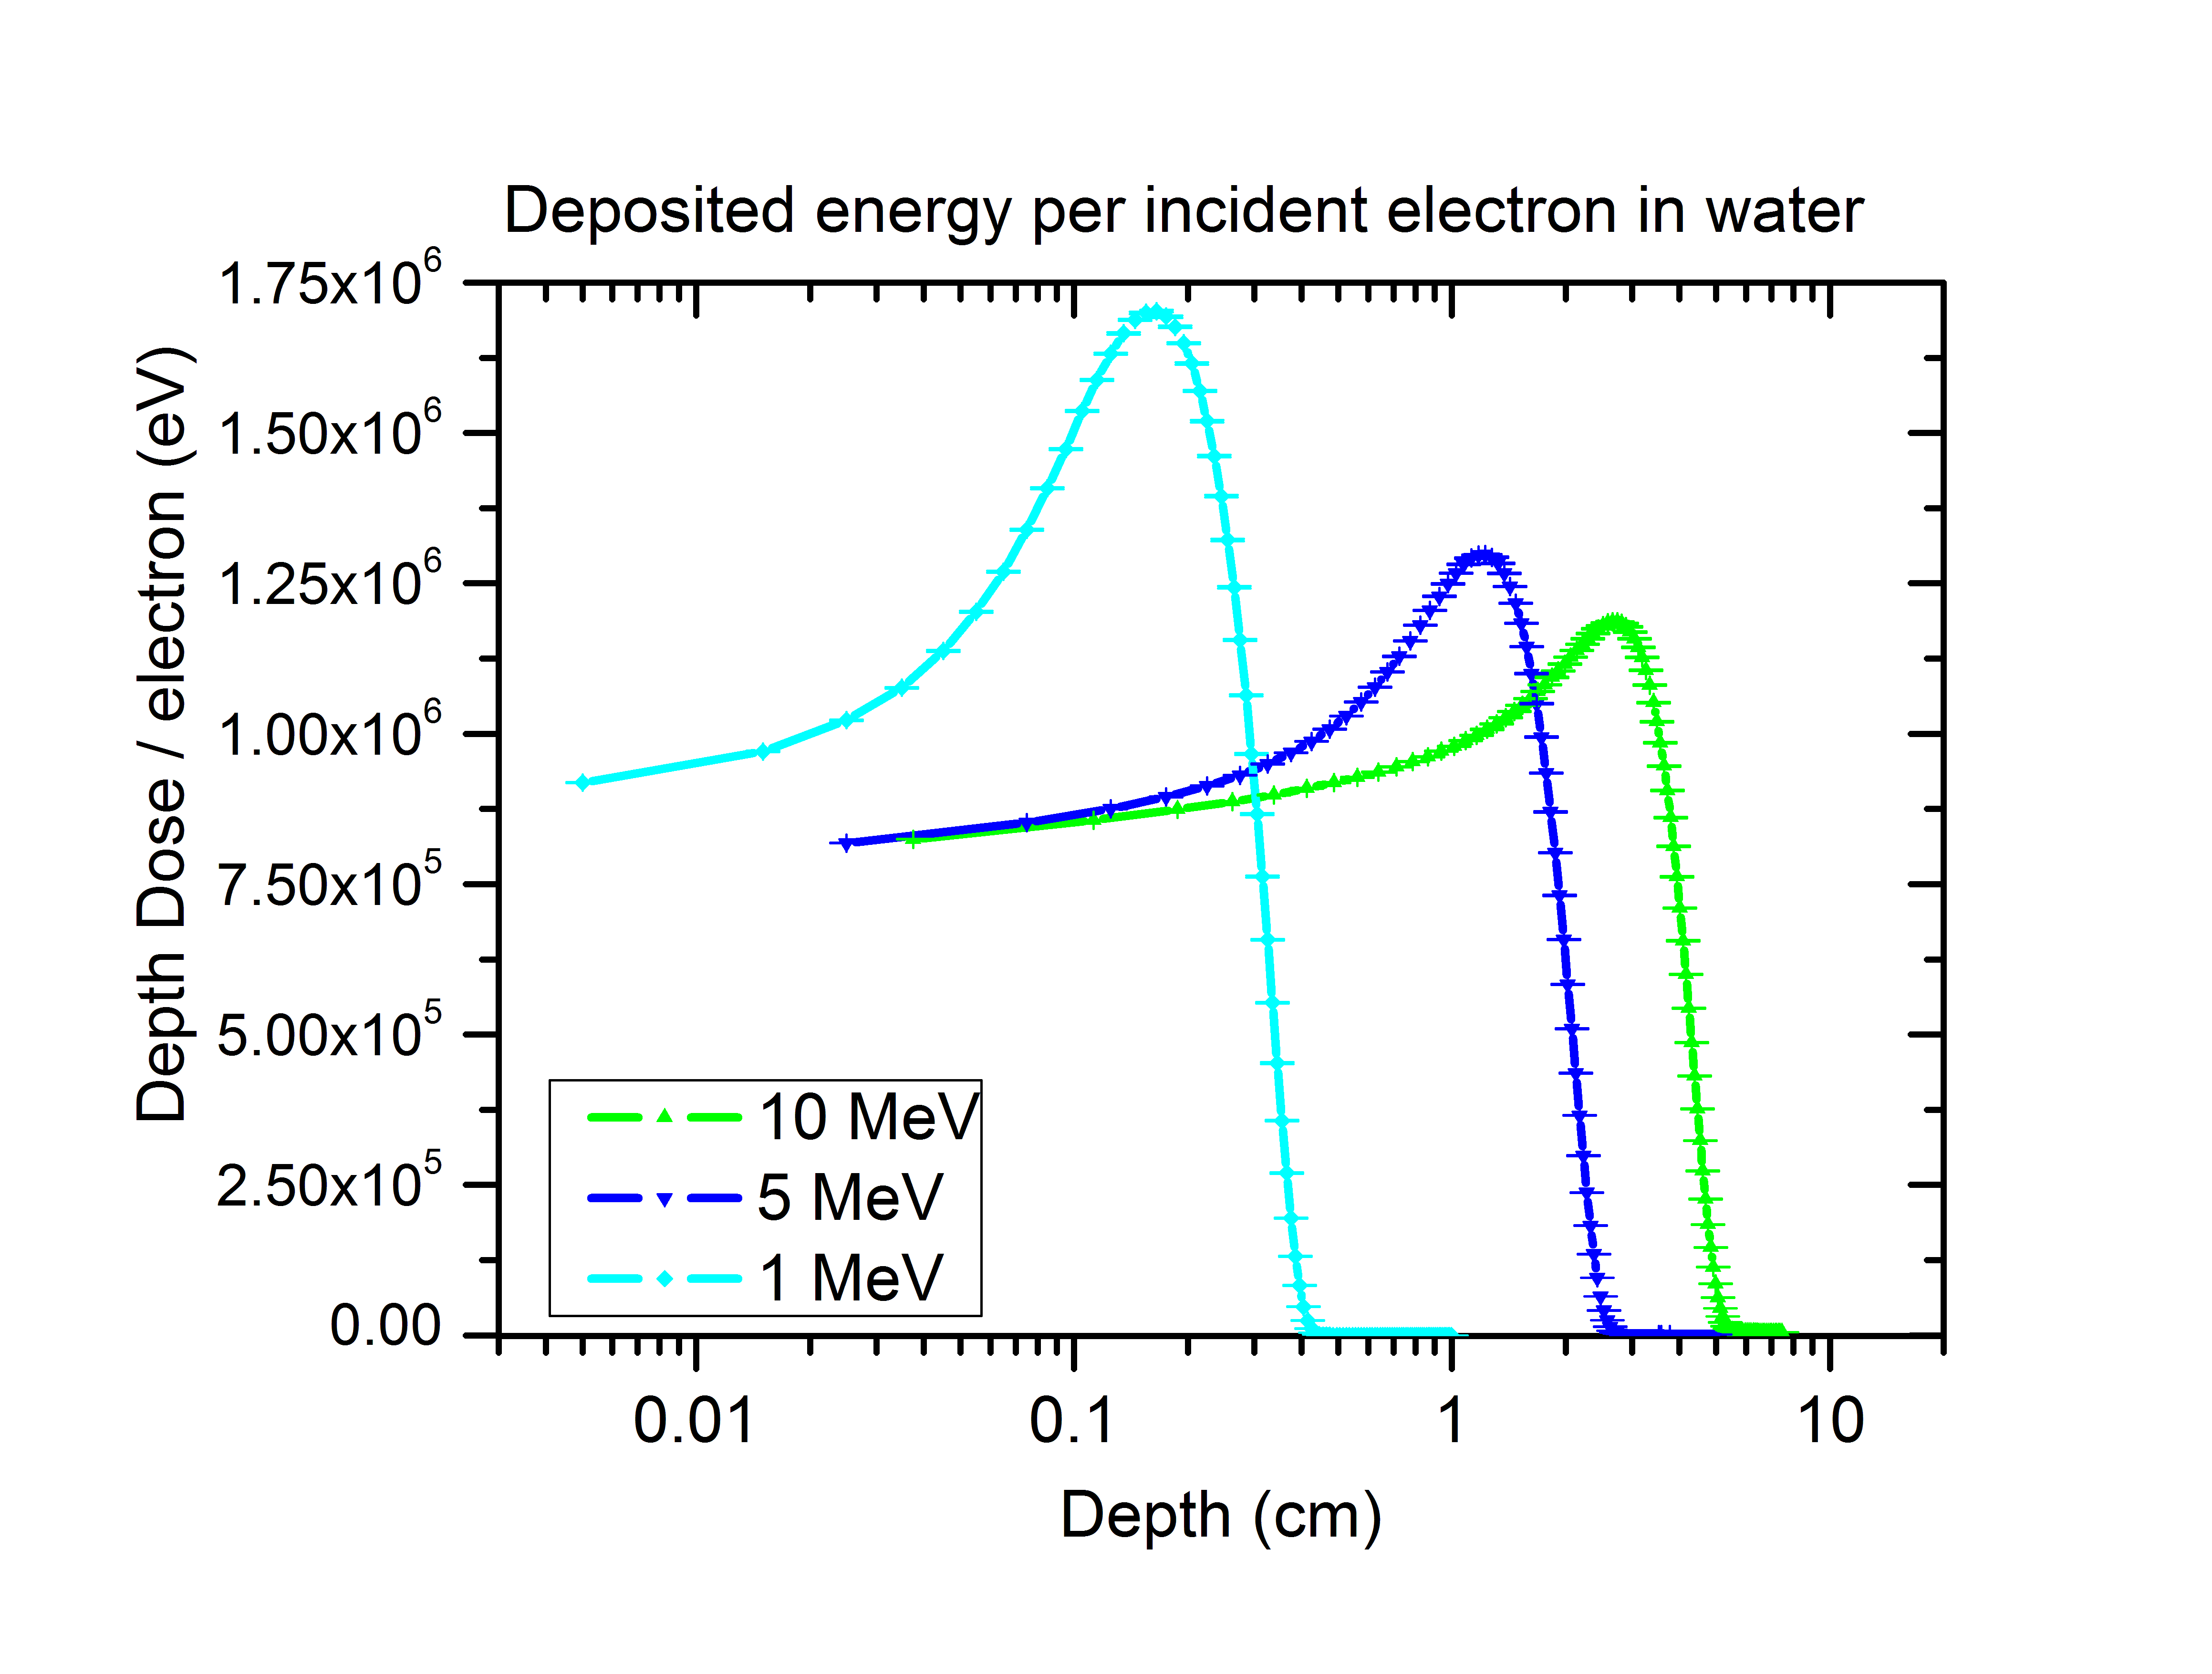
\includegraphics[width=\textwidth]{PENE_DepthDose.png}
			\caption{(a) Depth Dose}
		\end{subfigure}
		\begin{subfigure}[h]{0.5\textwidth}
			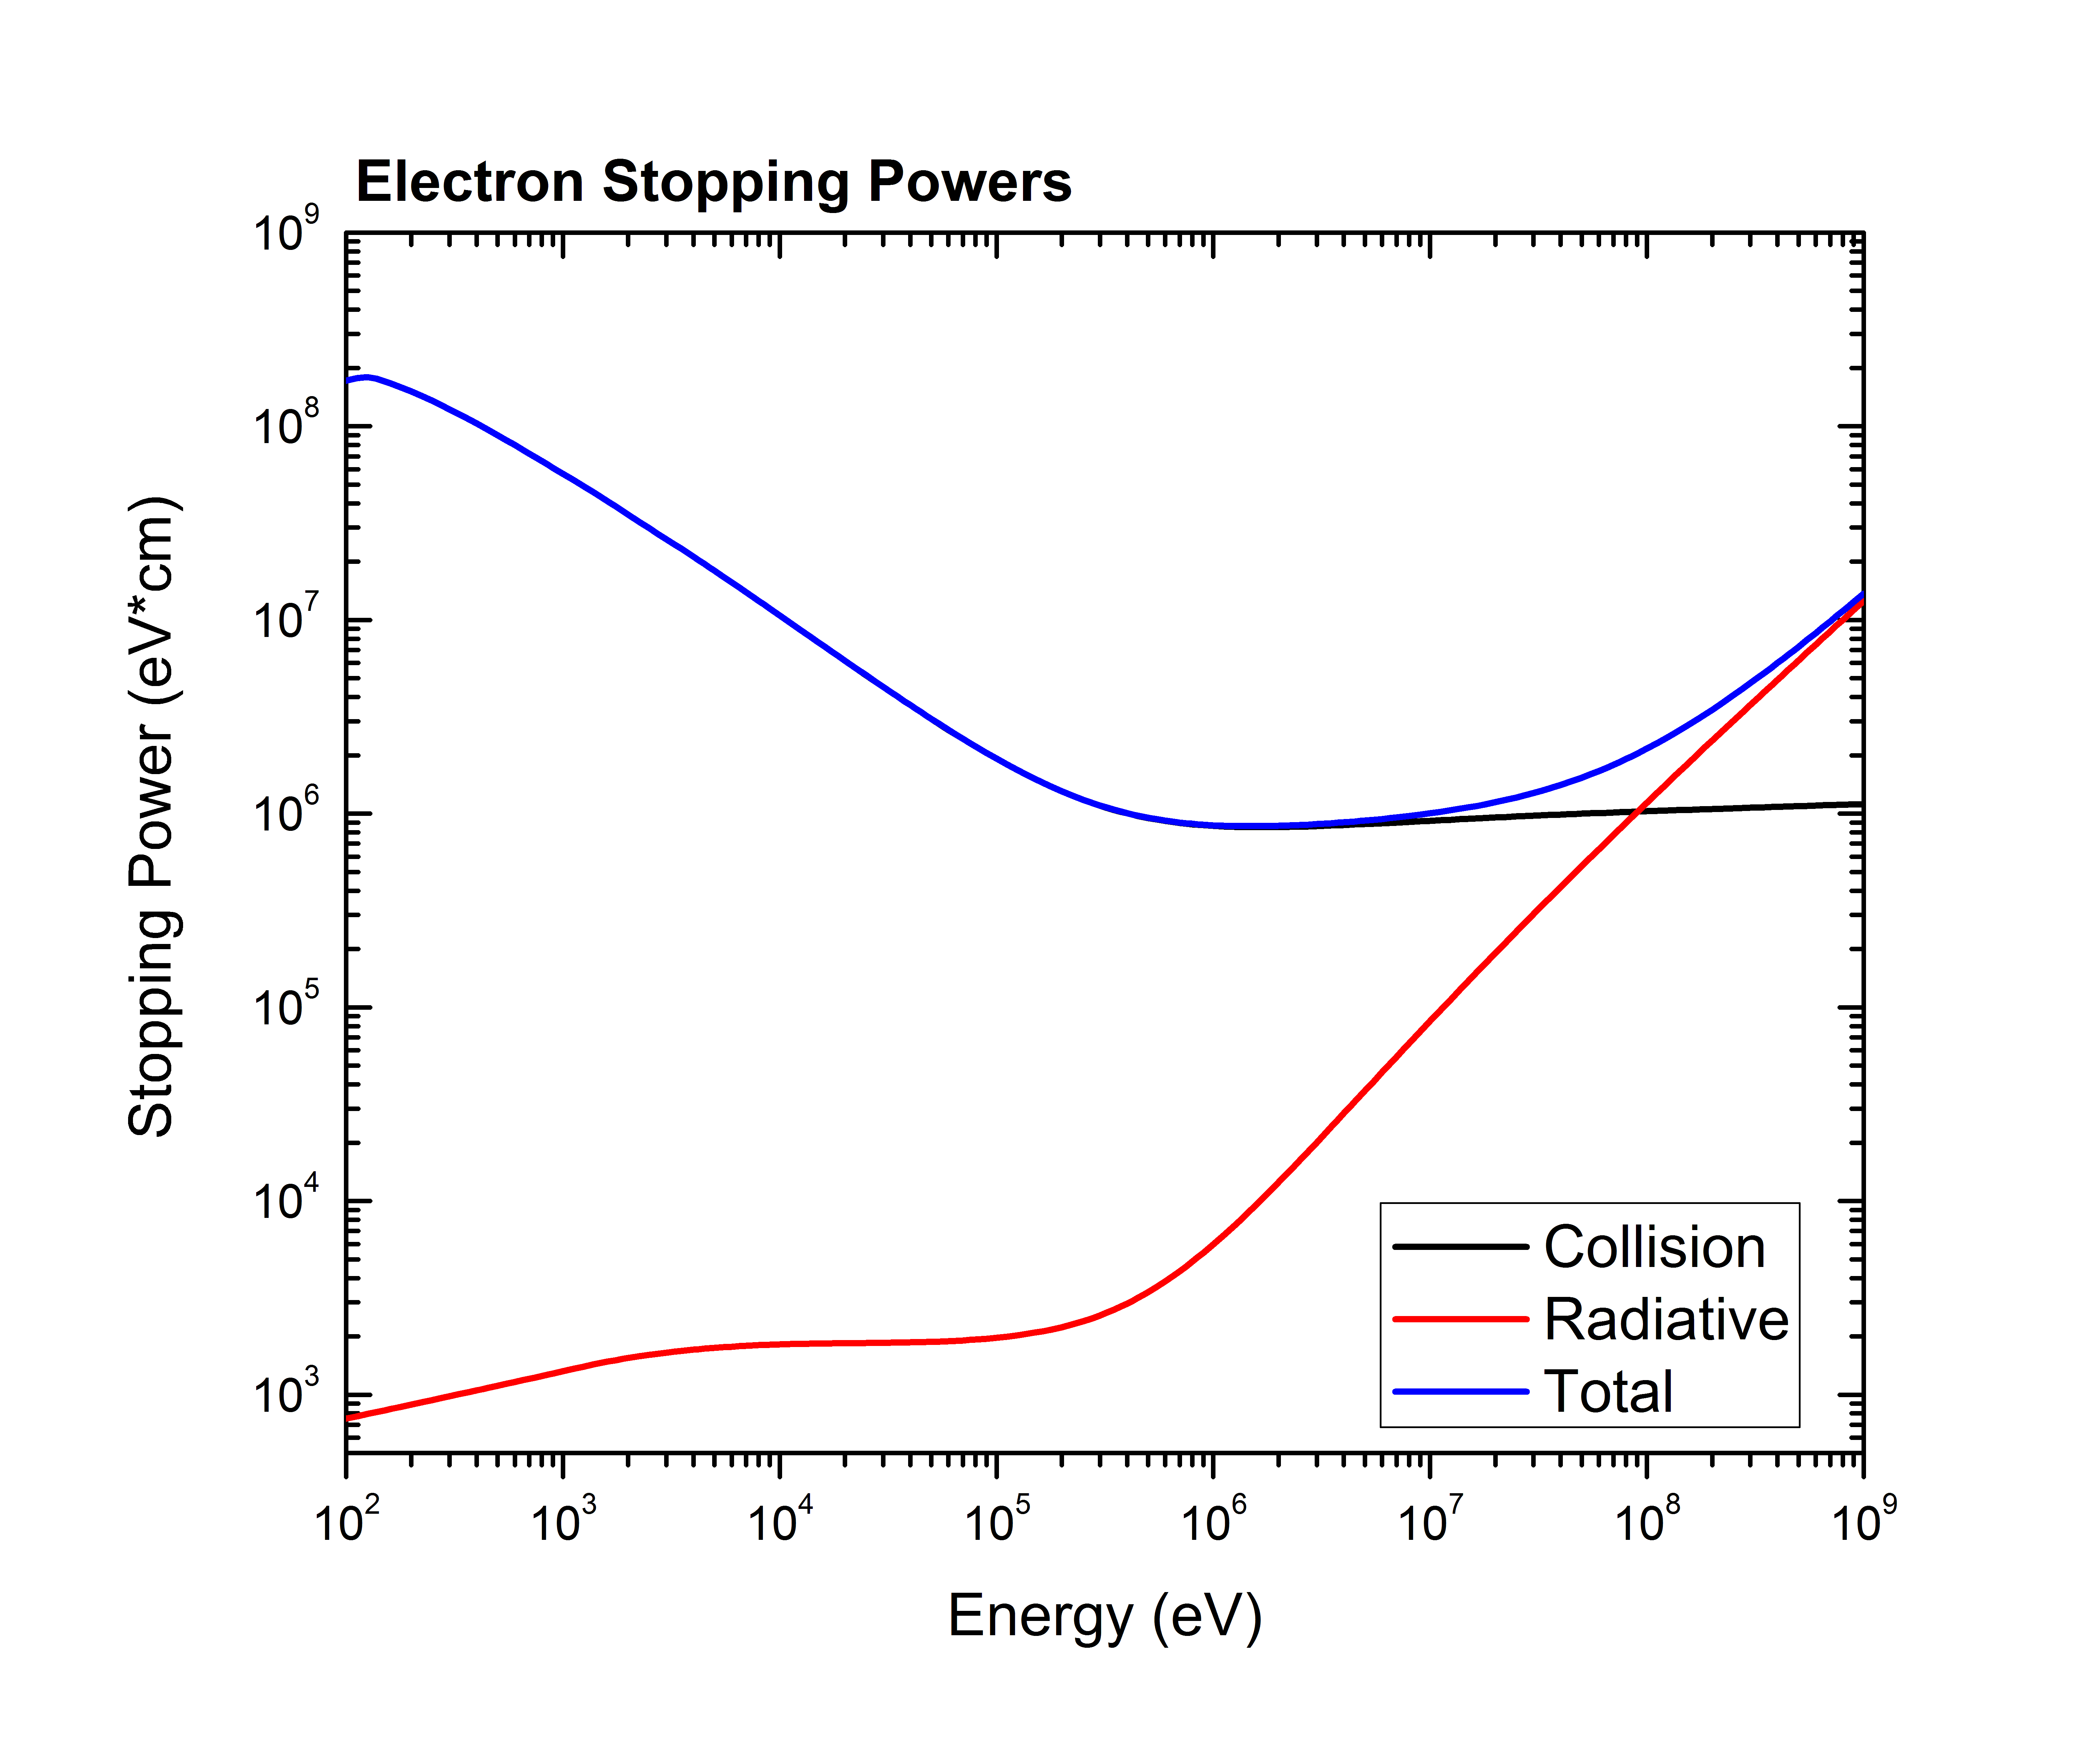
\includegraphics[width=\textwidth]{elec_stp.png}
			\caption{(b) Stopping Power}
		\end{subfigure}
		\begin{subfigure}[h]{0.5\textwidth}
			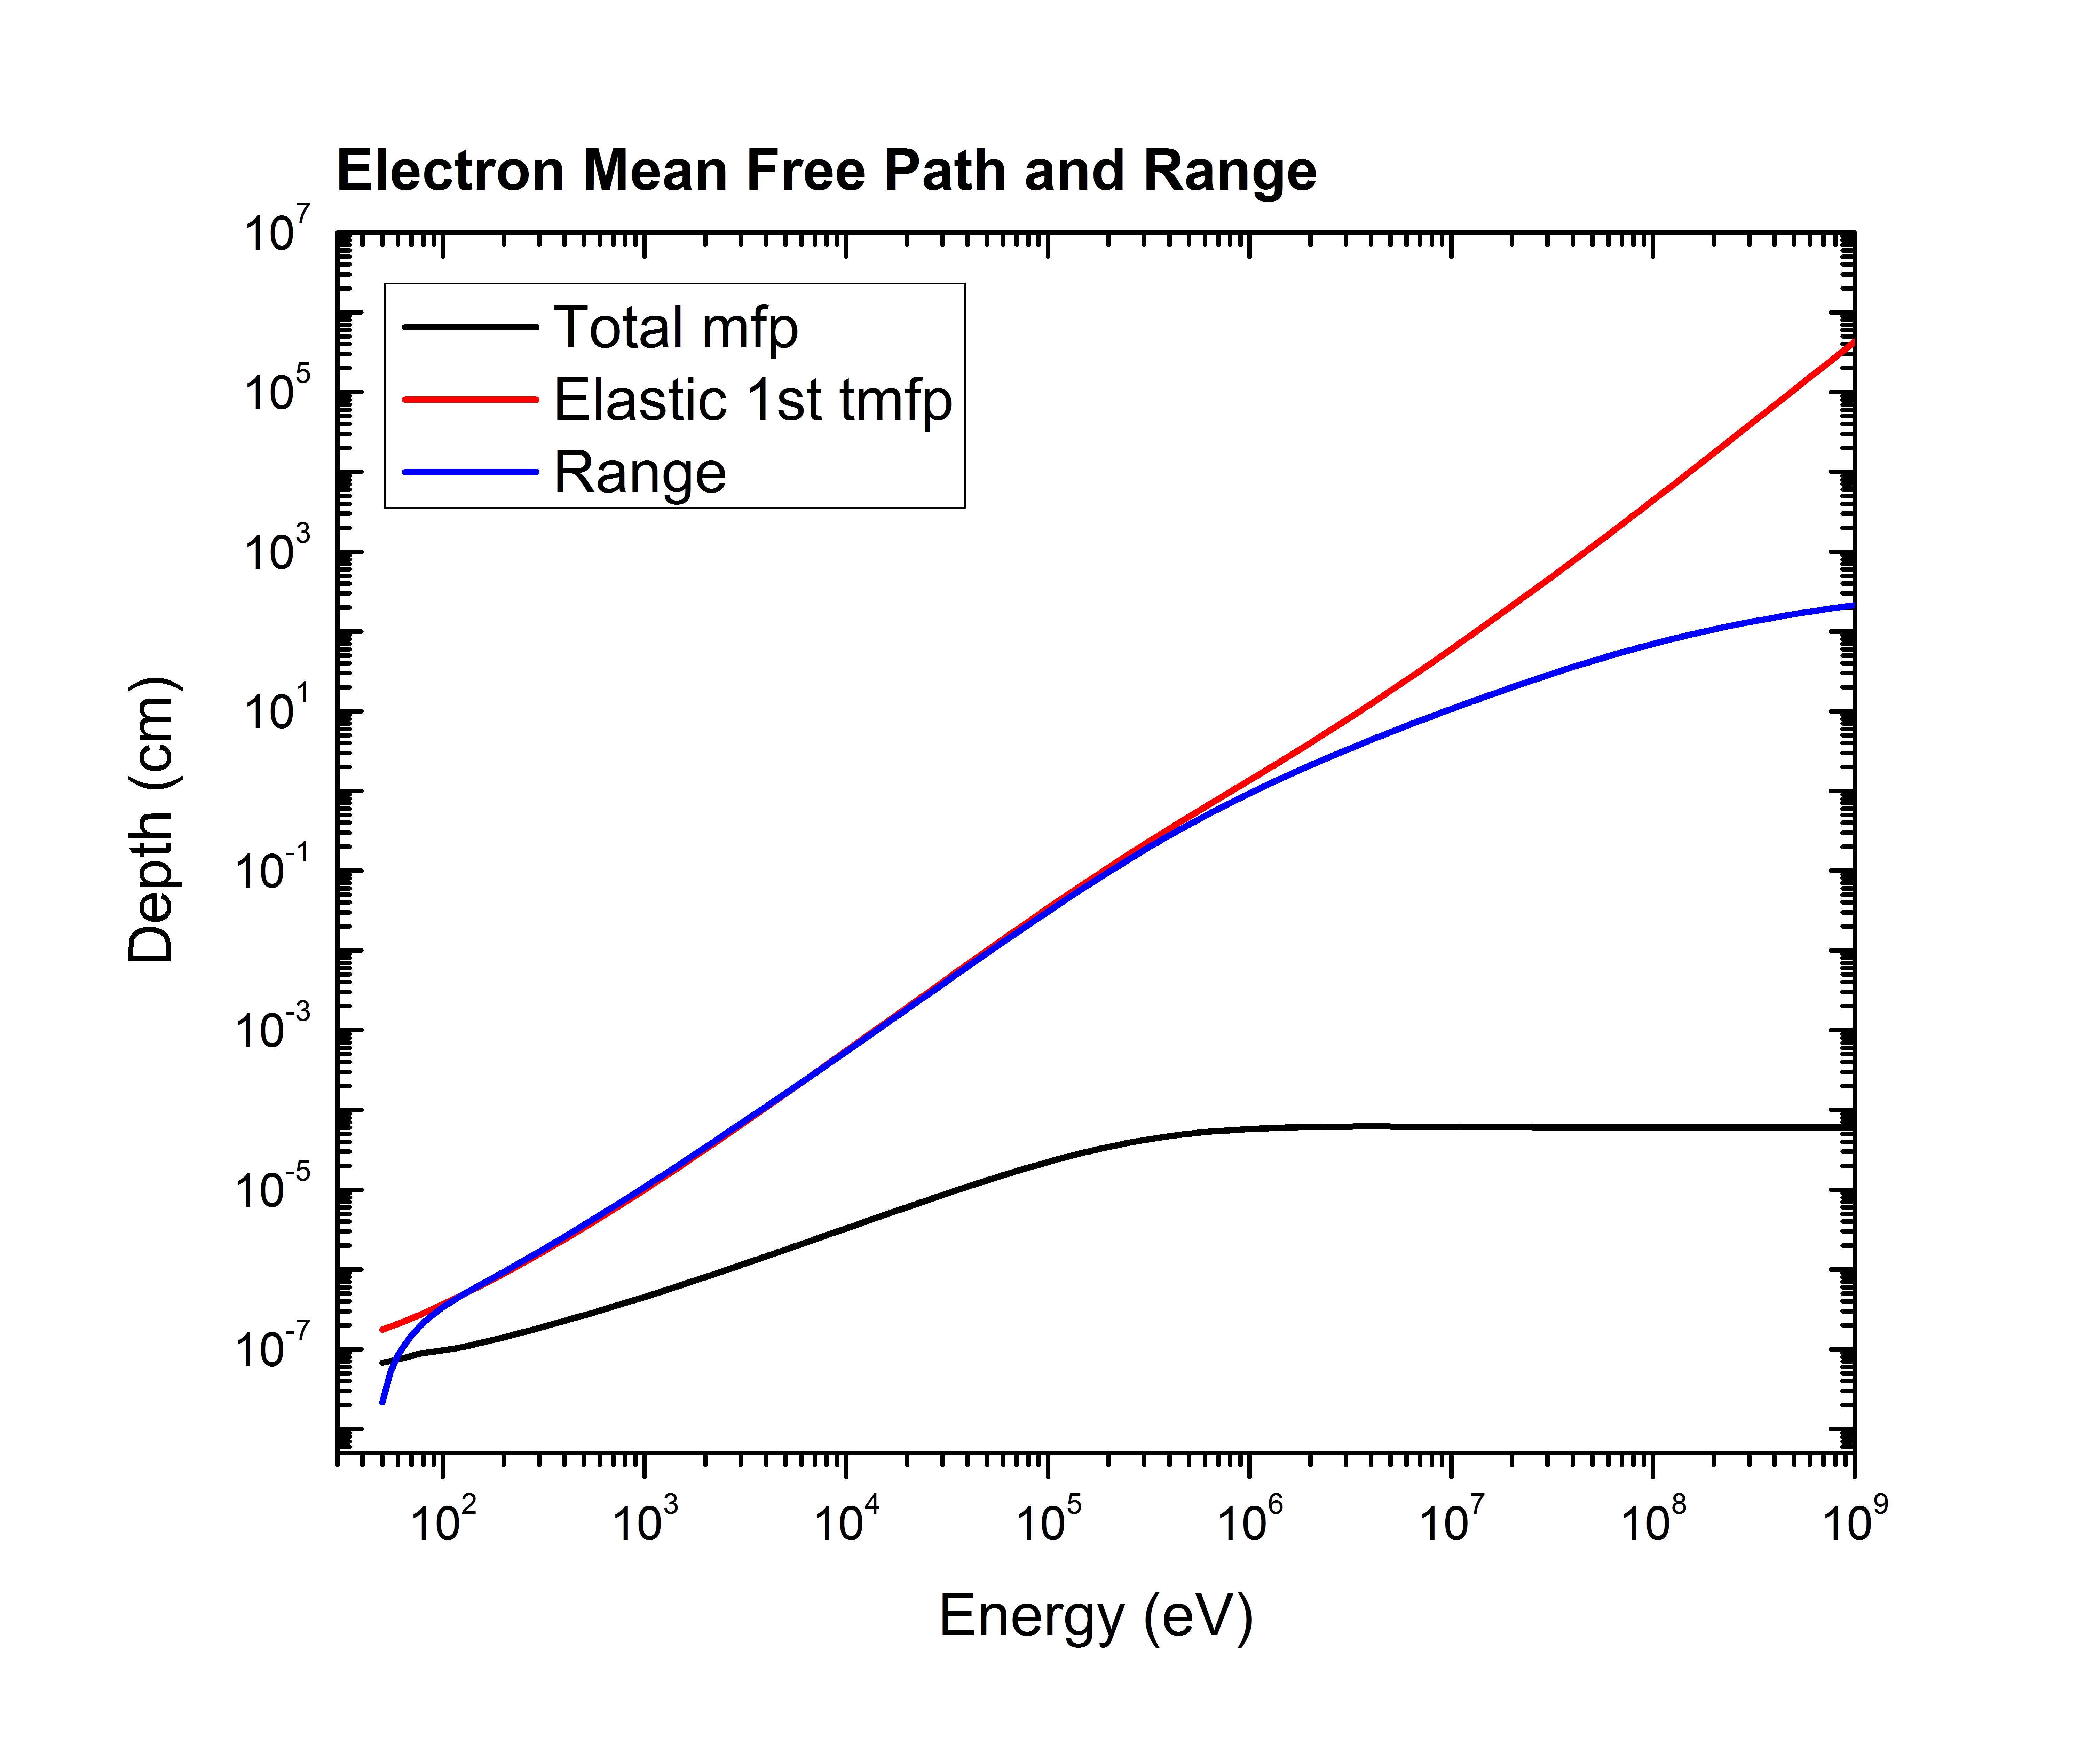
\includegraphics[width=\textwidth]{elec_range.png}
			\caption{(c) Projected Range}
		\end{subfigure}
		\begin{subfigure}[h]{0.5\textwidth}
			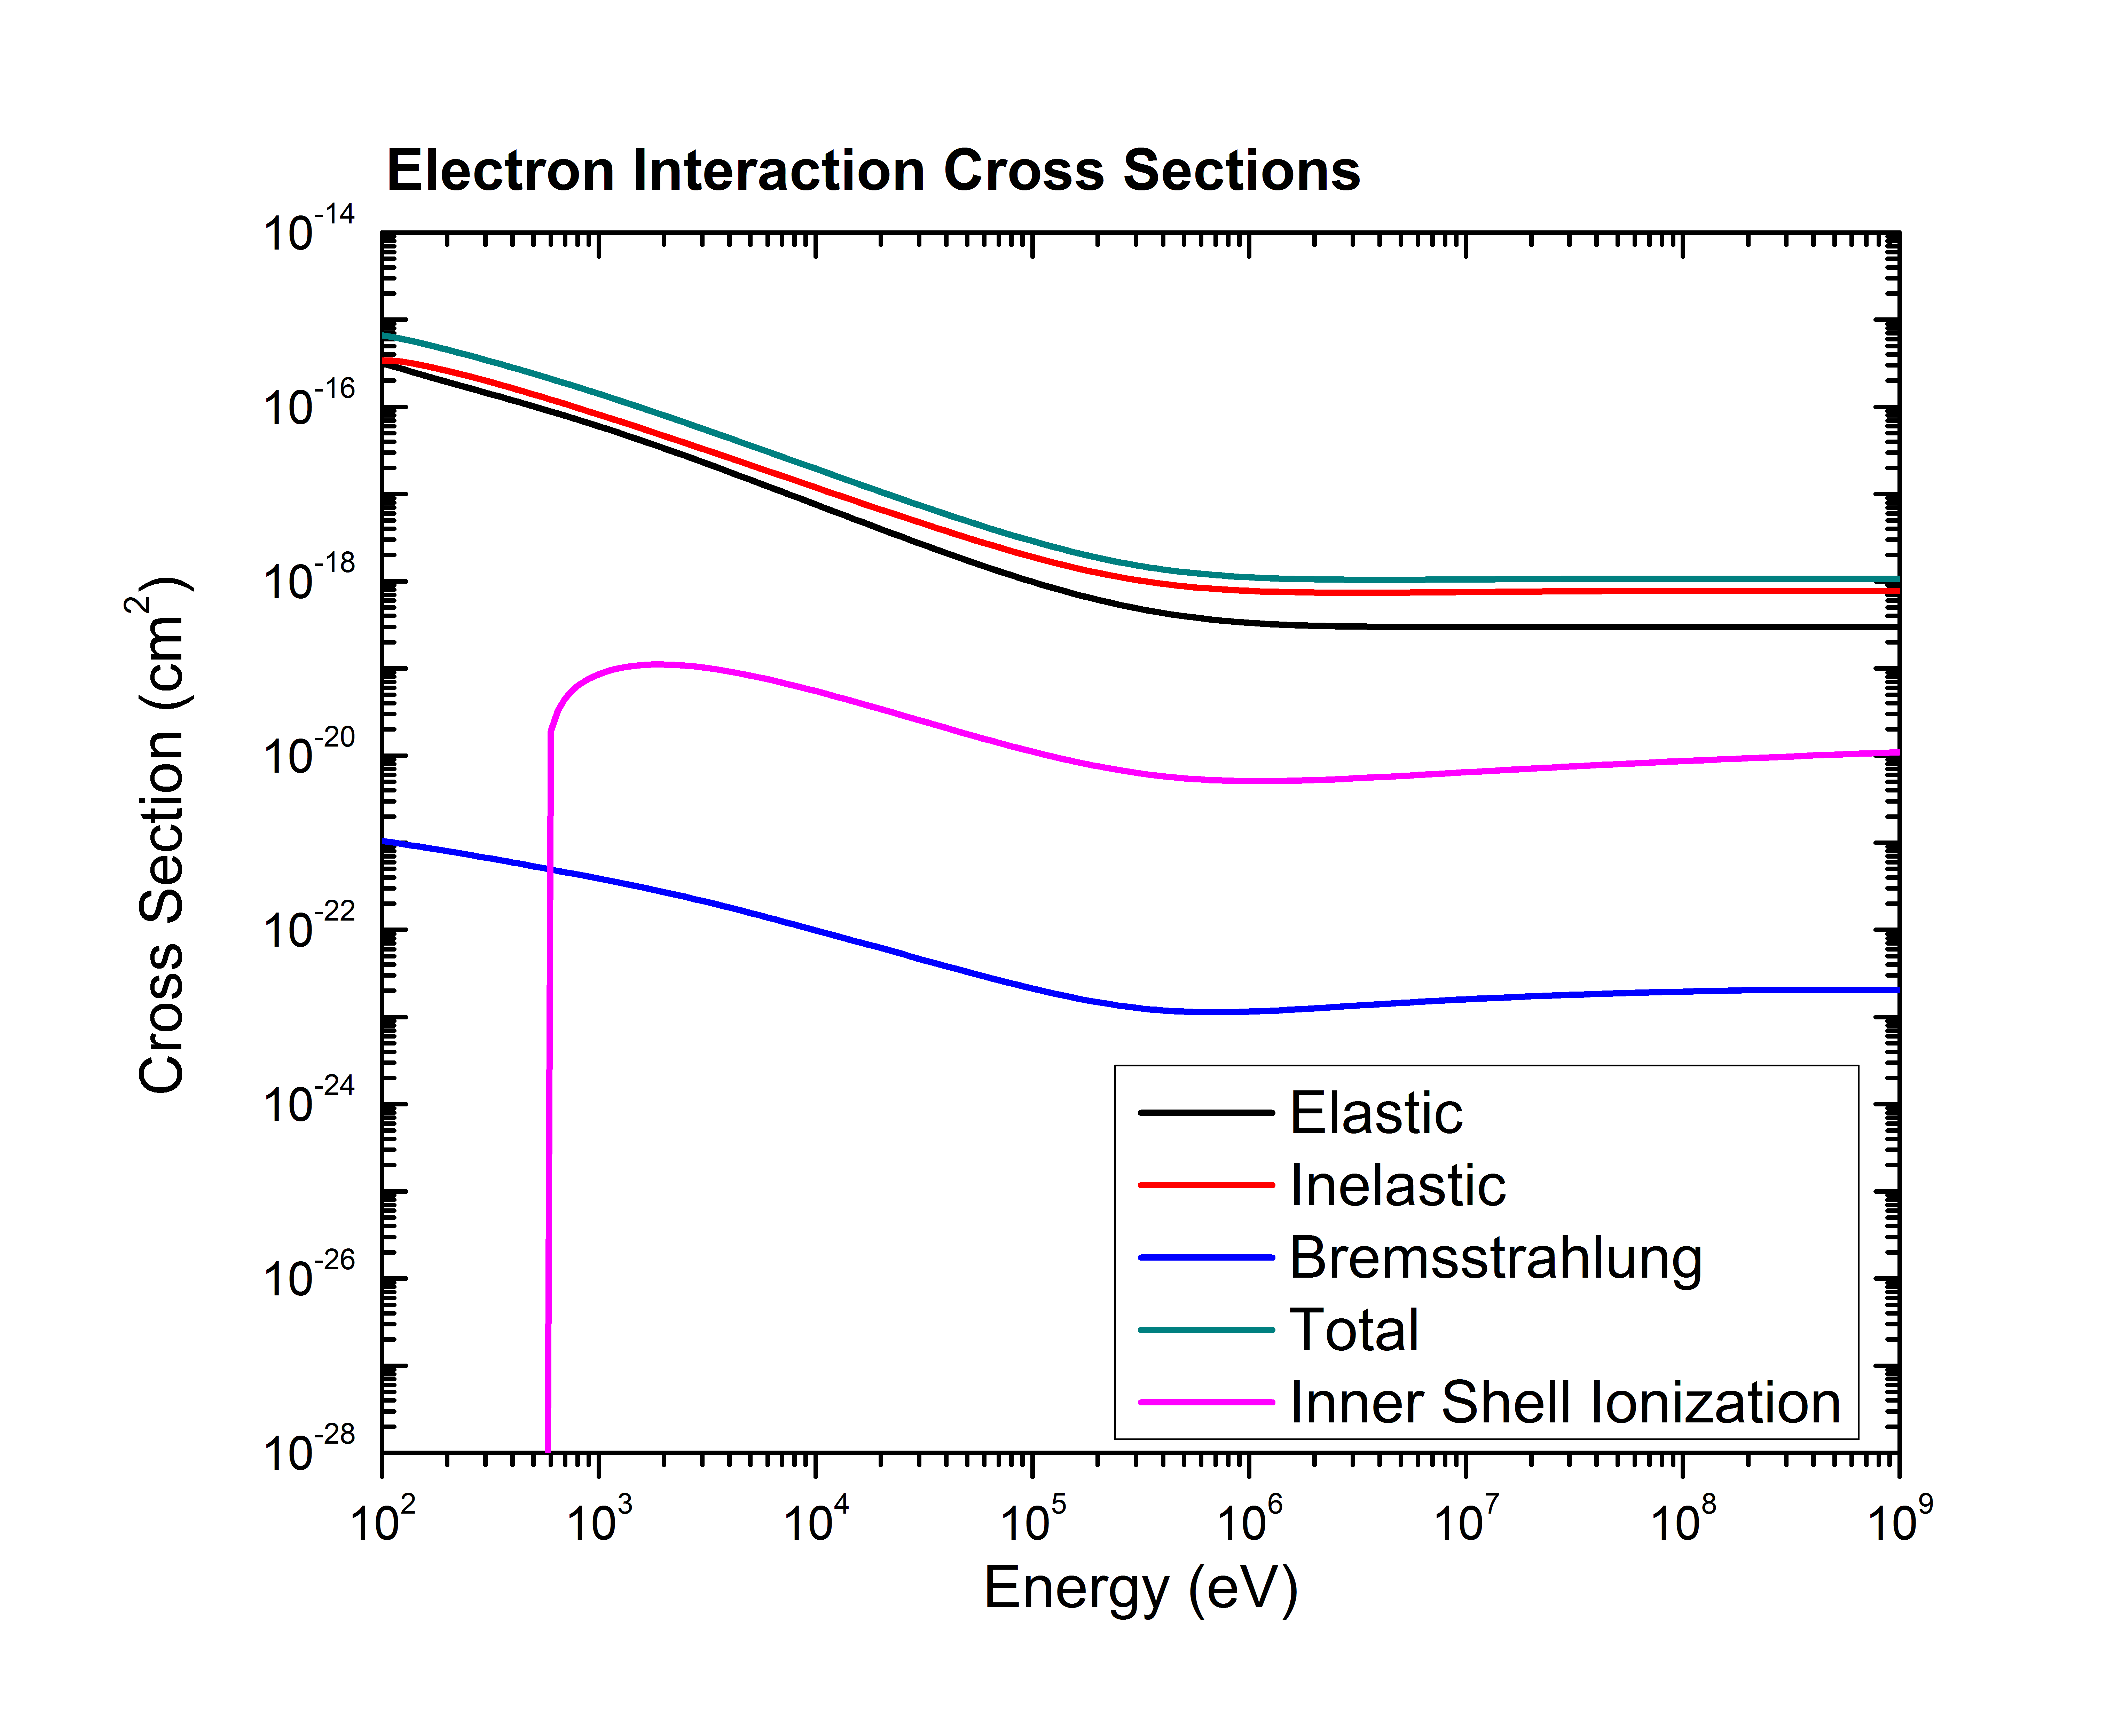
\includegraphics[width=\textwidth]{elec_xsec.png}
			\caption{(d) Cross Section}
		\end{subfigure}
	\caption{Electron energy deposition profile and stopping power calculated for pure water using the Penelope program [Salvat etal., 2011]. Simulations were run for xxx incident electrons and the results were scaled to a mean ice density of $\rho = \rho_{ice}(1-\phi)$ for $\rho_{ice} = 0.934 g/cm^{3}$ and $\phi=0.5$. (a) The depth-dose distribution D(z) is defined as the average energy deposited per unit depth per incident electron. D(z)dz is the energy deposited in a given interval and by integrating over the entire curve the incident electron energy is obtained: $E_{inc} = \int{D(z)dz}$. The statistical undertainty is given as $\sigma_{E(z)} = \sqrt{\frac{1}{N}\left[{\frac{1}{N}\sum{N}{i=1}c^{2}_{i,z}E^{2}_{z}}\right]}$. (b) The 'stopping power' is the mean energy loss per unit path length and is similar to a force slowing down the electrons. (c) The range gives the average penetration into the water ice. (At the moment I am not sure if this is projected depth or CSDA range, although I infer it is the latter.) (d) The cross-section gives the likelyhood of energy lost to a specific event or the average energy loss due to the different interaction processes (Elastic and Inelastic collisions (momentum transfer?), Bremmsstrahlung (negligible), and ionization).}
	\end{figure}
	
	The energy spectrum and expected deposition rate in the neighborhood of Mimas and Tethy's has been measured by the Cassini spacecraft and reported by Paranicas et al [2011, 2013]. Figure ~\ref{fig:ParanElec} shows the measured energy spectra and deposition profile taken from Paranicas et al. (2013).
	
		\begin{figure}[ht] \label{fig:ewater}
	\centering
		\begin{subfigure}[h]{0.5\textwidth}
			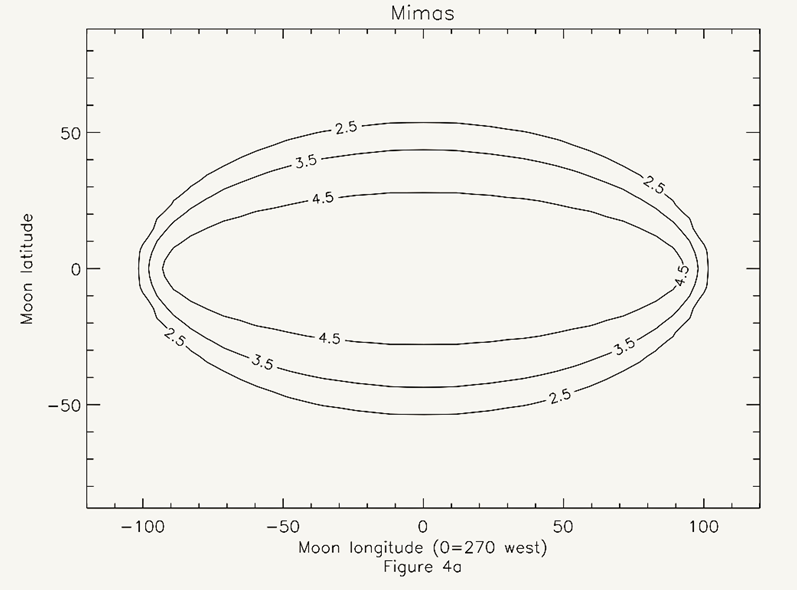
\includegraphics[width=\textwidth]{Paranicas_MimasDepositionProfile.png}
			\caption{(a) Mimas Deposition Profile}
		\end{subfigure}
		\begin{subfigure}[h]{0.5\textwidth}
			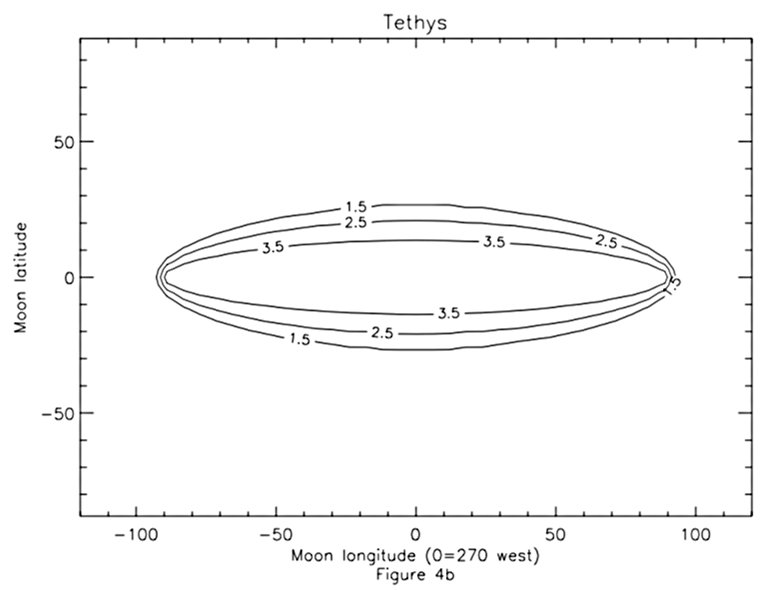
\includegraphics[width=\textwidth]{Paranicas_TethysDepositionProfile.png}
			\caption{(b) Tethys Deposition Profile}
		\end{subfigure}
		\begin{subfigure}[h]{0.5\textwidth}
			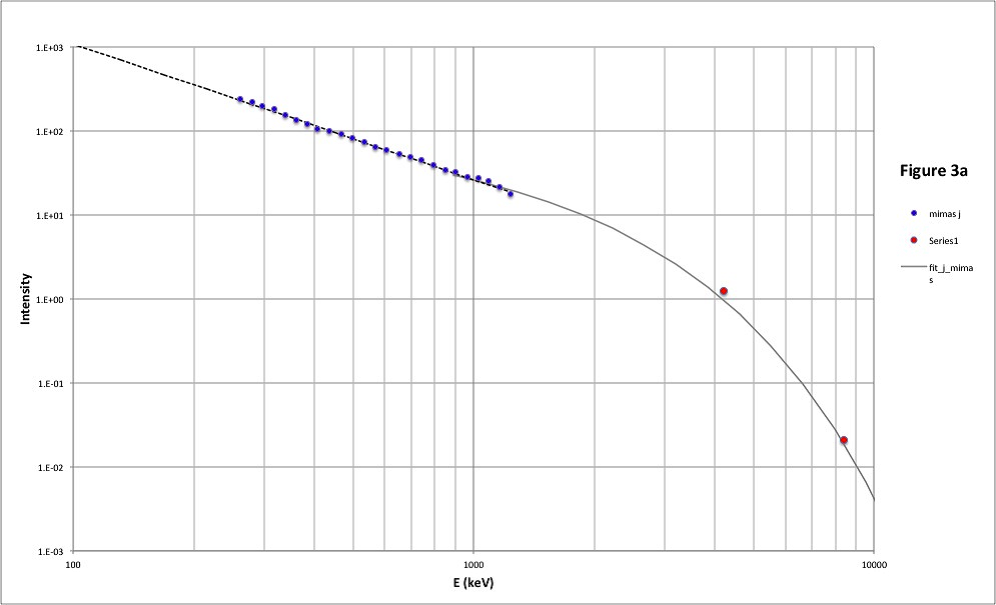
\includegraphics[width=\textwidth]{Paranicas_MimasEnergySpectrum.png}
			\caption{(c) Mimas Electron Energy Spectrum}
		\end{subfigure}
		\begin{subfigure}[h]{0.5\textwidth}
			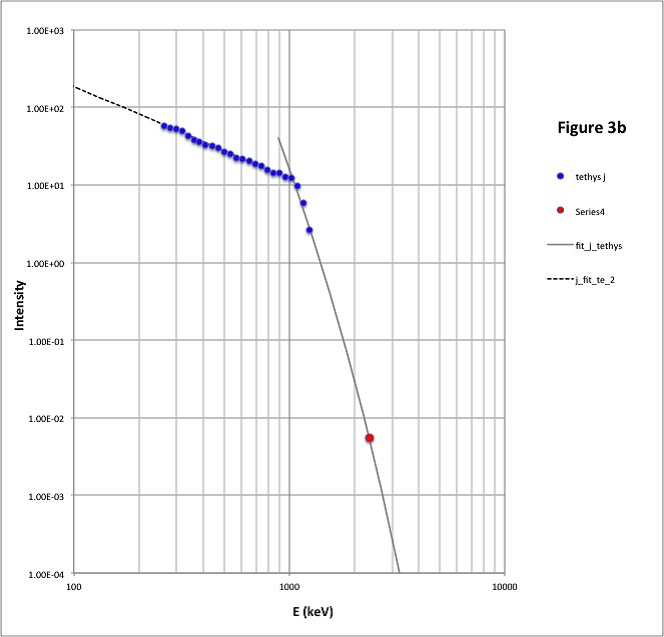
\includegraphics[width=\textwidth]{Paranicas_TethysEnergySpectrum.png}
			\caption{(d) Tethys Electron Energy Spectrum}
		\end{subfigure}
	\caption{Electron energy deposition profile and energy spectrum measured by the Magnetosphere Imaging Instrument (MIMI) on Cassini. Images were taken from Paranicas et al. [2013].}
	
	%REJ - Having the Paranicas energy distribution you can assume it heats the grains and use the average heating in sintering formula you have found Then we can also think about what individual excitations does in a grain with the energy spread over the grain and lost slowly by conduction. And then what a heat spike randomly distributed in a grain does.



% The production of excitations changes as a function of energy.
% What is the average energy deposition per grain vs. depth? \\
% What is the average temperature increase per grain vs. depth? \\
% What is the relaxation time for the grain to return to ambient temperature? Can this be calculated using measured thermal conductivity? \\
% What is the extent of diffusion to the sintering region that occurs during the heating events, vs. depth? \\
	
	The similarity in the penetration depths of the electrons and the skin depth of the thermal anomaly suggest that the electrons could be responsible for the increased thermal conductivity.  Here we consider that a possible explanation for the thermal conductivity differences is sintering between adjacent regolith grains driven by energy deposited in electronic excitations of the water molecules either near the surface or in the bulk of the ice grains. The deposited energy can mobilize water molecules, causing them to migrate along the grain surface, through the bulk, or desorb from the surface and reabsorb in the intergrain region. This can lead to grain growth and, more importantly, growth in the size of the contact regions between grains and improved thermal contact  across the grain boundaries.
	
	 As discussed below the same energy deposition that mobilizes the water at the grain boundaries can cause defects in the bulk. Whereas sintering increases the effective thermal conductivity, such defects, which we assume to be the principal cause of the increase in the IR/UV ratio[ref], can cause a decrease in thermal conductivity. Below we will also show that the density of bulk defects produced at a level consistent with the sintering are sufficient enough to affect the UV scattering but not to significantly decrease the thermal conductivity.
	
%\emph{There should be a pressure minimum in the pendular region. Need equation to explain. Another argument is the minimization of surface energy. Need to look more into that too.}
	
\section{Contributions to the effective thermal conductivity of an icy porous regolith}

	In general, the effective thermal conductivity of a granular, uncemented sample under vacuum can be separated into a conductive component which describes heat flow through the bulk and a radiative term which describes heat flow through the void space [Watson, 1964]. 
	
	\begin{equation} \label{eq:TCbasic}
	k_{eff} = k_{rad}(T^{3}) + k_{cond}
	\end{equation} 
	
	The first term depends on both grain size and porosity and is due to radiation as discussed further below. The second factor was given by Watson (1964) as $k_{cond} = \frac{3000}{r_{g}}\times10^{-5}$ for $r_{g} > 20 \mu m$ and is a function of the bulk conductivity of the grain material ($k_{g}$) and the contact area ($S$) between grains. For cold, porous regoliths typical of airless solar system bodies in the outer solar system, heat flow is limited by the amount of intergrain contact.

	In general, $k_{rad}$ and $k_{cond}$ can depend on factors such as grain size, porosity, temperature, packing structure etc. Additionally, molecular desorption and feedback heating can raise the gas pressure in the pore space giving an additional convective path for heat transfer between grains ($k_{conv}$). Thermal conductivity measurements and modeling using either a spherical grain approximation or continuum techniques can be used to parameterize the variables for analytical expressions. However, much work has been done to constrain the various parameters that affect the thermal conductivity, and those possibly relevant to Mimas and Tethys will be outlined and their usefulness for describing the effective thermal conductivities reported by Howett et al., (2011, 2012) is discussed below.
	
%	Computationally, though variations in porosity, vacuum conditions, and grain size can be difficult to study in the lab and using solid sphere computational models may miss important effects from the regolith microstructure.

\subsection{Radiative contribution to thermal conductivity}

	The contribution to the effective thermal conductivity from radiative heat emission from the grain/pore surfaces, $k_{rad}$, can be estimated as [Kasparek and Vortmeyer, 1976]

	\begin{equation}
	k_{rad} = 4 \psi r_{g} \sigma T^{3}
	\end{equation}
	
	where $r_{g}$ is the particle diameter, $T$ is the temperature, $\sigma$ is the Stephan Boltzmann constant, and $\psi$ is a heat transport coefficient defined by
	
	\begin{equation}
	\psi = \frac{2F + \epsilon'(1-F)}{2(1-F)-\epsilon'(1-F)}
	\end{equation}

	for which F is a 'radiative constant' equal to $\approx$ 0.08 and $\epsilon'$ is related to the emissivity $\epsilon$ of the material by $\epsilon' = \frac{\epsilon}{\epsilon +0.5(1-\epsilon)}$. Taking $r_{g} = 50 \mu m$, and $\epsilon = 1$, then the radiative contribution to the thermal conductivity can be estimated as $k_{rad} \approx 6.3\times10^{-6} \frac{J}{m \cdot s \cdot K}$.
	
	Thus we see that the radiative contribution at approximate Mimas temperatures can account for only $\approx 1/3000$th of the total thermal conductivity as measured for the anomalous region on Mimas. Though it could account for as much as 1/10th of the thermal conductivity outside of the anomalous region on Tethys, it is typically on the order $<1\%$ contribution to the total thermal conductivity and will be neglected in the remainder of our analysis.

\subsection{Latent heat contribution to thermal conductivity}
	An additional mechanism not considered by Watson (1964) in Eq.\ref{eq:TCbasic} is heat transfer due to molecular desorption and re-absorption within pores, i.e. sublimation, the expectation being that there is a higher rate of sublimation on the high temperature side of the pore and thus heat conductivity across the void space. We can model the contribution from the sublimation process using the Hertz-Knudsen formula [ref]:

	\begin{equation}
	k_{lat} = ( \frac{\mu}{2 \pi k_{B} T})^{1/2}  (L S) \frac{dP}{dT}
	\end{equation}
	
	where $m$ is the molar mass of the gas molecule, $k_{B}$ is the Boltzmann constant, $L$ is the latent heat of sublimation per unit mass and $S = \phi r_{g}$ is the average pore size dimension where $\phi$ is the porosity and $r_{g}$ the average particle diameter. The vapor pressure $P$ of the gas of interest is given by the Clausius-Clapeyron equation:
	 
	 \begin{equation} \label{eq:CCpres}
	 P = ae^{(-b/T)}
	 \end{equation}
	 
	 where $a$ and $b$ are experimentally determined parameters for water vapor over ice given by Fanale et al. (1984) as $a = 3.56 \times 10^{13} dyne/cm^{2}$ and $b = 6141.667 K$. Taking the latent heat of sublimation to be $L = 48600 [\frac{J}{mol}]$ and again using a temperature of 80 K, the contribution to thermal conductivity from the latent heat is $k_{lat} = 1.15\times10^{-26} MKS$. Though at low temperatures this effect is negligible, Steiner and K\"{o}mle (1991) showed that it should be included at temperatures above ~170K. At the temperatures considered here the net thermal conductivity of the grains is controlled the second term in Eq.\ref{eq:TCbasic} and is modeled as due to solid state heat transfer.

\subsection{Solid state heat transport and contact area effects}
	There are several methods in the literature for estimating solid state heat transfer in a grainy regolith that take into account grain size, porosity, and a cementation or contact area between adjacent grains. For cold grainy regoliths, heat flow is limited by the intergrain contact area which in turn depends on the crystallinity and defect structures of the cementation region or grain boundaries. Considering reasonable parameters for water ice grains, the contact radius can be obtained directly through Hertzian analysis. Alternatively, by considering a 'Hertz-factor' that scales the bulk thermal conductivity to account for reduced heat flow at grain contacts and taking the measurements of effective thermal conductivity for the moon surfaces and making reasonable assumptions about packing structure, porosity, grain size, and thermal conductivity of the grain materials, the relative contact area between grains in the areas inside and outside the anomalous region can be compared for the various models. 
	
%	Then it can be determined if the energy deposition from the MeV electrons is sufficient to explain the larger relative contact area within the anomalous region.
	
	One of the major differences in the following models is that some include the Hertz factor (contact area radius) to only the first power [Wood, 2013; Gundlach and Blum, 2012], while the other models include the square of the contact radius [Kossacki et al., 1994; Sirono and Yamamoto, 1997]. The models also differ in their dependence on regolith grain size. 

\subsubsection{Hertz-factor description of grain contact area}
	In modeling of thermal conductivity of grainy and porous materials, a common approximate technique is to consider a mono- or poly-dispersed 'bed' of elastic spheres. The requirement for the spheres to be elastic and not a perfect hard sphere stems from physical considerations, since the contact point of hard spheres is infinitesimal, through which no heat can flow, meaning that the spheres must deform slightly at the contact point so there is some finite area across which heat can flow. At the atomic scale, the heat transfer through dissimilar spheres with no rigid bonding is due predominantly to the van der Waals interactions which mediate the phonon transfer, while for cemented grains heat is conducted directly through lattice vibrations. Deformation between curved, elastic surfaces in contact was first studied by Heinrich Hertz in 1882, and Hertzian analysis can be used to determine the intergranular contact area and indentation depth of the surfaces. The contact radius between two spheres depends on the material properties and is related to an applied load $F$ by:

	\begin{equation}
	R_{con,eff} = \left[ \frac{3}{4} \frac{1 - \nu^{2}}{E(T)} r_{g} F \right]^{1/3}
	\end{equation}

	where $\nu$ and $E(T)$ are Poisson's ratio and Young's modulus of the material, respectively. The applied load determines how strongly adjacent particles are bonded and, for a loose regolith, the weight of the grains can be used to determine the force and thus the contact area. However, gravitational forces in the near surface region are negligible as compared to van der Waals bonding which provides orders of magnitude greater adhesive interactions. The adhesive force is effectively the tensile load at the point where the spheres are separated and can be calculated by JKR theory [Johnson et al., 1971].
	 
	 \begin{equation}
	 F_{JKR} = 3 \pi \gamma_{s} r_{g}
	 \end{equation} 
	 
	 where $\gamma_{s}$ is the specific surface energy of the material at the solid/vapor interface. Hertzian analysis can be used in thermal conductivity expressions for non-cemented grains to describe the effective radius of the intergranular contact and make comparisons for otherwise identical regoliths to determine the relative area through which heat can flow. A larger contact radius corresponds to greater interparticle contact, thereby allowing a greater heat flux and a higher thermal conductivity. It should be noted here that these expressions may not be applicable for cemented grains where the intergrain boundary may have some degree of crystalline bonding. Instead, thermal conductivity in these instances can be modeled by taking into account of cementation area which will continue to be the limiting factor in heat transfer through the regolith grains. 
	 
	 %REJ -  we can comment on the uncertainties in the grains sizes  -- but lets focus on the increase in the contact area and try to model how that could occur due to the radiation. I think we have to go more quickly to the approximations that you believe commenting on the estimates that did not lead to much useful and focusing on what you believe.

	Assmuing the water grains are spherical and taking parameters typical of ice at $\sim-5\degree C (\gamma_{ice/ice} = 65 mJ/m^{2}$ [Ketcham, 1969], $\mu_{ice} = 0.33$, and $E_{ice} = 9 MPa$ [Hobbs, 1974] $)$, the contact force ($F_{JKR}$) for zero volume fraction cementation and the effective contact radius ($R_{con,JKR}$) can be calculated for $50 \mu m$ grains (Tab.\ref{tab:HertzGrain}). Taking the Hertzian contact radius to be linearly related to be the ratio of the effective and bulk thermal conductivities as a dimensionless 'Hertz factor' $k_{eff} = k_{ice}(R_{con}) = H k_{ice}$ we can determine the relative thermal resistance of the surface regions. Further assuming materials parameters as well as the packing structure are the same inside and outside the anomaly so that the only difference is grain size, the ratio necessary to explain the measured thermal conductivity differences can be determined. 
	
	\begin{align*}
	\frac{k_{eff,in}}{k_{eff,out}} \varpropto \frac{H_{in}}{H_{out}} \varpropto \left( \frac{r_{g,in}}{r_{g,out}} \right)^{2/3}
	\end{align*}
	
	Although most authors take the dependence on the Hertz-factor to be linear [Wood, 2013; Gundlach and Blum, 2012; Steiner and K\"{o}mle, 1991] as above, it is also interesting to interpret the Hertz factor more directly as the radius of the contact area between grains and take differences between the bulk (crystalline ice) and effective (measured) thermal conductivity to be related by the contact area between grains  - $k_{eff} \varpropto (R_{con})^{2} (similar to Sirono and Yamamoto (1997), although they took $k_{eff} \varpropto (r_{g})^{-2/3}). 
	
	\begin{align*}
	\frac{k_{eff,in}}{k_{eff,out}} \varpropto \left( \frac{R_{con,in}}{R_{con,out}} \right)^{2} \varpropto \left( \frac{r_{g,in}}{r_{g,out}} \right)^{4/3}
	\end{align*}
	
	It should be noted that as it stands, $k_{eff} ~ k_{ice}\cdot R_{con}^(2)$ does not balance units. Various authors approach this differently, but typically some form of "structure factor" or dependence on the cementation neck radius is assumed. The neck typically has a pendular form due to surface energy minimization restrictions [Piqueux and Christensen, 2009b; Kossacki et al., 1994; *Dvorkin*]. 
	
	\begin{table}[h] \label{tab:HertzGrain}
	\caption{JKR adhesion force and Hertzian contact radius calculated using the surface energy and mechanical properties of $\sim -5 \degree$ water-ice grain sharing boundaries with vacuum and adjacent grains. Taking the Hertz factor as the ratio of the effective and crystalline ice thermal conductivities we can determine the relative grain size of the different surface regions for both linear and quadratic dependence on the contact radius.} 
	\centering
		\begin{tabular}[c]{| c | c | c | c | c | }
		$F_{JKR}$ & $R_{con,JKR}$ & \multicolumn{1}{| c|}{} & $\multicolumn{2}{c | }{$\frac{r_{g,in}}{r_{g,out}} } \\ \cline{4-5}
		[N] & [$\mu$ m]& \multicolumn{1}{| c|}{} &  Mimas & Tethys \\ \hline 
		\multirow{2}{*}{$3.06\times 10^{-5}} & \multirow{4}{*}{4.84} & $k_{eff} \varpropto R_{con}/r_{g} & $2.08\times10^{-4}$ & $6.43\times10^{-5} \\ \cline{3-5}
%		 & & $k_{eff} \varpropto (R_{con}/r_{g})^{2} & $0.0144$ & $0.008$ \\ \hline 
		 & & $k_{eff}\varpropto (R_{con})^{2}$ & $8.32$ & $11.17$ \\ \cline{3-5}
%		 & & $k_{eff}\varpropto (R_{con}$) & $69.26$ & $124.7$ \\ \cline{3-5}
		\end{tabular}
	\end{table}
	
	\emph{I have to admit that at this point I feel sure I must be making a mistake in my analysis of the various models. Can they really treat grain size dependence so differently? Need to double check these relationships in detail while going through the various TC models.}
	
% 	THIS WAS MY PREVIOUS ESTIMATE AND SEEMS TO BE VERY WRONG. IT THERE STILL A MISTAKE BEING MADE? MUST DOUBLE CHECK!!!	At lower temperatures where radiative heat transfer is negligible, the thermal conductivity $k_{eff} \varpropto (r_{g})^{-1/3}$ and will increase with decreasing particle size, possibly due to the increased number of interparticle contacts. Taking the ratio of the grain sizes inside and outside the anomaly on Mimas, we find
	
%	\begin{equation}
%	\frac{r_{g,in}}{r_{g,out}} = (\frac{R_{con,out}}{R_{con,in}})^{3} = 0.00013
%	\end{equation}
	
	(Need to propagate errors) Taking $k_{eff} \varpropto (r_{g})^{-1/3}$ the grain size differences are much too large to be able to account for the thermal conductivity differences, while for $k_{eff} \varpropto (r_{g})^{-2/3}$ the relative size difference is the opposite what was measured for Mimas (larger grains inside the anomaly). Linear dependence on the contact radius yields the grain size comparison estimates where the particles within the anomaly are larger than that outside by two or three orders of magnitude. Considering instead a quadratic dependence on the contact radius the grain size difference is ~10, similar to the upper limits determined from UVIS measurements [Hendrixetal2012]. However, since no other authors considered in this study use a 4/3 dependence on the grain size, justification for this would be necessary. % *In a non-exhaustive search, I couldn't find that Howett et al ever discussed the relationship between grain size and thermal conductivity. Hendrix published Mimas grain sizes in 2012, while Howett discussed Mimas in their 2011 paper.*

\subsubsection{Continuum Modeling}
	 Intergrain heat conduction was studied by Piqueux and Christensen (2009) using a finite element code and assuming a pendular cementation region connecting grains. Though they were primarily concerned with the effect of gas pressure in the voids between grains, their results also considered low gas conductivities ($<1 \times10^{-5}$) which approach the thermal conductivity of a regolith in a vacuum.
	
	\begin{figure}[h] \label{fig:PCresults}
	\centering
		\subfloat{{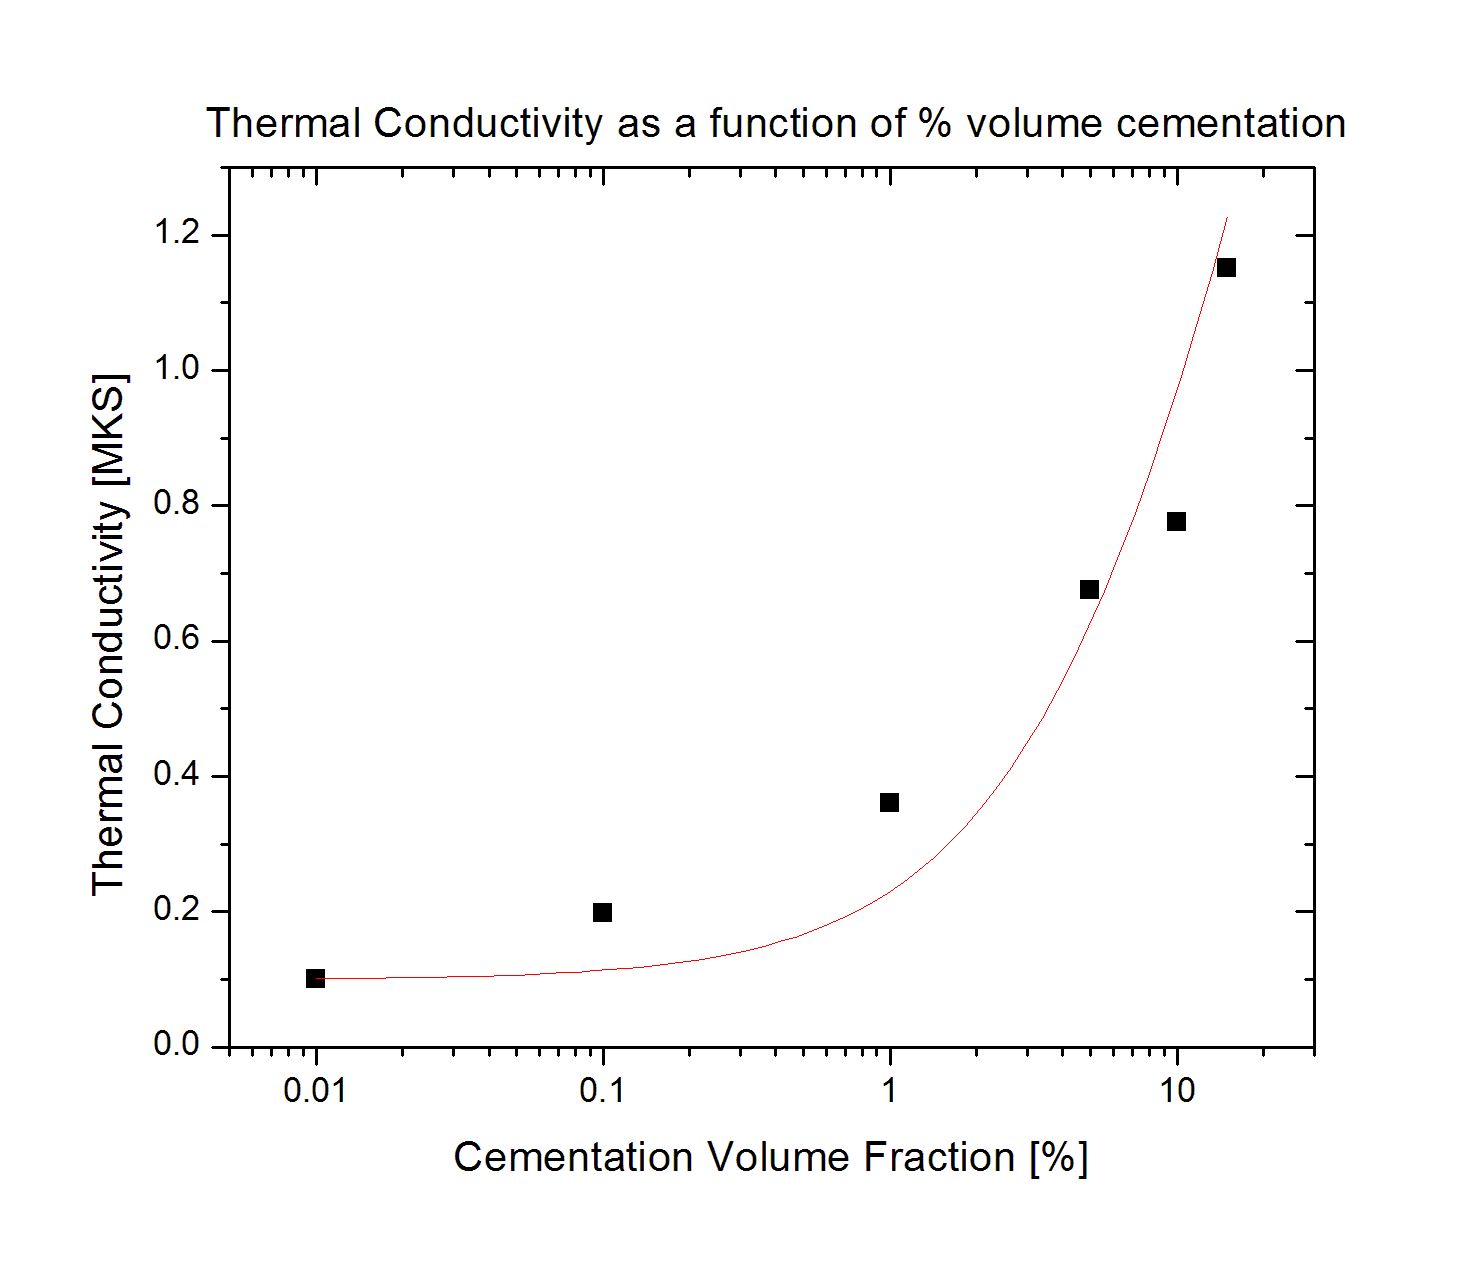
\includegraphics[width=0.57\textwidth]{PandQ2009b_CemVolumeFraction.png} }}
		\subfloat{{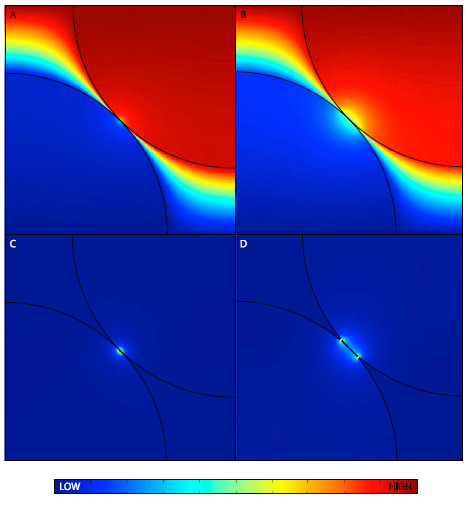
\includegraphics[width=0.43\textwidth]{PandQ2009b_Temp_grainimage.png} }}
		\caption{(Left) Thermal conductivity as a function of \% volume cementation for a 33\% porous grainy regolith. The red line represents a logarithmic fit to the data (add equation to image).  (Right) Relative temperature (a and b) and heat flux (b and c)  in a cubic centered cell from finite element numerical modeling results. Panels a and c are for a cell without bonding, and b and d represent a 0.01\% by volume pendular ring connecting the grains. The thermal conductivity of the cementation and grain material was taken to be 6 MKS and 0.937 MKS and for the interstitial gas it was 0.003 MKS in both cases. Data taken from Piqueux and Christensen (2009).}
	\end{figure}

	Figure \ref{fig:PCresults}.1 shows that the thermal conductivity of the anomalous region on Mimas ($k_{eff, in} = 0.0113$ MKS) falls well below the minimum cement volume fraction considered in the modeling. The relationship between the cement volume fraction and thermal conductivity can be approximated by $k_{eff} \varpropto \cdot ln(1.105 \pm 0.177 + VF_{cem}\cdot 0.154 \pm 0.177)}$, and it can be seen that, for vanishing gas conductivity, the volume fraction of cement ($VF_{cem}$) inside the anomaly should be $<1\times10^{-6} \%$. In fig.\ref{fig:PCresults}.2d shows that the heat flux with 0.01\% volume cementation is concentrated toward the edges of the cemented area, while for no cementation (fig.\ref{fig:PCresults}.2b) the heat flux is concentrated at the point of contact. 
	
	Important differences between these simulations and the regolith of Mimas and Tethys are that the packing structures investigated were all cubic regular packings and the grain thermal conductivity used was 0.937 MKS, much lower than for water ice and typical of basaltic glasses. However, the cement thermal conductivity used was 6 MKS, typical of crystalline ice, and since heat transfer of cemented grains is dominated by the cementation material the lower thermal conductivity of the grain should not be cause significant affect the thermal conductivity of the grain boundary region. *Grain thermal conductivity may play a more important role in determining the thermal inertia of an icy regolith due to the time scales involved.* It was shown that for very low cement volume fractions the cement thermal conductivity is negligible and the effective thermal conductivity, for the ranges of \% volume cementation evaluated, approaches a single value dependent on grain size and pore gas pressure. Though the effect of varying the grain thermal conductivity was not discussed in the paper, it can be assumed to be negligible given that heat transfer between grains is limited by the point of contact. Since the small cementation volume fractions of the order estimated by extrapolation to the low thermal conductivies of Mimas and Tethys were not considered, this model may not be sufficient to explain the small boundary conduction changes due to electron heating of grains.

\subsubsection{Maxwellian effective conductivity}
	 Wood (2011, 2013) developed a heat transfer model for grainy porous regolith based on the Maxwell equation for effective conductivity of an isotropic, heterogeneuos media. Although originally developed for electrical conductivity, the equation applies equally to thermal conductivity where the thermal paths - solid state conduction, convection through gas filled pores, and radiation from grain surfaces across pores - can be taken as acting in parallel as in Eq.\ref{eq:TCbasic}. The conductive term takes into account both solid and gas phase heat transfer and is limited depending on which phase forms a continuous path throughout the material, the lower limit corresponding to a continuous gas phase and the upper limit to a continuous solid phase. Since the lower limit is strictly valid only when the solid particles are not in contact, a non-physical situation for a regolith material, the degree of solid phase continuity is taken into account by introducing a multiplicative factor. Taking the radiative term to be negligible as discussed above, the effective thermal conductivity is given as
	
	\begin{equation}
	k_{eff} = k_{cond,min} +f_{sc}(k_{cond,max}-k_{cond,min}).
	\end{equation}
	
	For the low pressure environments of Mimas and Tethys the lower thermal conductivity limit can be taken to be zero. The upper limit depends on the thermal conductivity of the grain material $ k_{g}$, the porosity $\phi$, the volume percent and thermal conductivity of cementation region, $\chi$ and $k_{cem}$ respectively, and the fractional continuity of the solid phase $f_{sc}$. Assuming that the cementation and bulk grains are both crystalline ice ($k_{g} = k_{cem} = k_{ice}$) and that the volume percent cementation is much less than the grains ($\chi << 1-\phi$), the effective thermal conductivity becomes:	
	
	\begin{equation}
	k_{eff}=2 f_{sc} k_{ice} \frac{1-\phi}{2+\phi}
	\end{equation}
	
	The $f_{sc}$ factor represents the effect of interparticle contact and/or cementation and is a measure of the efficiency of contact between adjacent grains. The factor contains both geometrical and contact area considerations and, for uncemented soils, is given in terms of the size and number of contacts per particle, where contact size is determined by Hertzian analysis and cohesive surface forces (JKR theory).
	
	\begin{equation}
	f_{sc} = Y_{sc}N_{c} \left( \frac{N_{c}}{2\sqrt{N_{c}-1}} \frac{R_{con}}{r_{g}} \right)^{Z_{sc}}
	\end{equation}
	
	where R$_{con}$ is the radius of the contact area, r$_{g}$ is the grain radius, N$_{c}$ is the coordination number, Y$_{sc}$ is a factor determined by fitting to experimental data, and Z$_{sc}$ determines how the heat flux varies with contact radius between particles. Batchelor and O'Brien (1977) showed that the length scale for significant surface and bulk temperature variations is 
	
	$\lambda_{\nabla T} \approx \frac{r_{g}}{\alpha_{k}}$ 
	
	where 
	
	$\alpha_{k}=\frac{k_{cond}}{k_{conv}+k_{rad}}$
	
	When $R_{con} >> \lambda_{\nabla T}$, most of the heat flux is concentrated on the perimeter of the contact area and the effective thermal conductivity depends only linearly on the contact radius ($\Rightarrow Z_{sc} = 1$, see Fig.\ref{fig:PCresults}). However, when $R_{con}<\lambda_{\nabla T}$ the heat flux density is constant across the contact area and the total heat flux increases as the square of the contact radius ($\Rightarrow Z_{sc} = 2$). For the case considered here, the gas and radiative thermal conductivities are quite small meaning that $\alpha_{k}$ is large and $Z_{sc} = 1$. This differs from other thermal conductivity models considered below where the thermal conductivity is assumed to depend on the square of the contact radius. 
	
	 The coordination number can be calculated exactly for regular packings of monodisperse spheres, with N$_{c}$ = 6 for simple cubic packing which has a porosity of 47.64\%, similar to the porosity used here. For polydispersed mixtures of randomly packed particles the coordination number cannot be known exactly, but for small, cohesive, nearly spherical particles Yang et al (2000) gave a functional relationship between coordination number and porosity which closely matches measured and modeled random packings, especially at porosities $\ge40\%$. 
	
	\begin{equation}
	N_{c} = 2.02 \left( \frac{1+87.38(1-\phi)^{4}}{1+25.81(1-\phi)^{4}} \right)
	\end{equation}
	
	Using a porosity of 50\%, we find the coordination number is N$_{c}$ = 4.99. We note that for non-spherical particles the shape, orientation, and roughness of a particle can have an effect on the number of contacts and thus the porosity is less strongly coupled to the coordination number. The equilibrium contact radius between two elastic spheres of the same radius R$_{s}$ under a mechanical load can be calculated from JKR theory (Johnson et al., 1991) and is discussed in more detail for non-spherical particles by Wood (2013). An averaged best fit value of Y$_{sc}$ = 0.09 with a mean standard deviation of 13.6\% was found by fitting thermal conductivity data a variety of glass bead samples of various size distributions. Using these values and assuming a mean particle size of 50$\mu$m, we can determine the solid continuity factor, the effective contact radius, and the relative difference in contact inside and outside the anomalous regions. These values are given in Table\ref{tab:Wood2013}. 
	
	\begin{Table} \label{tab:Wood2013}
	\caption{Effective grain contact radius and ratio between inside and outside the anomalous regions as calculated using the theory of Wood 2013. Fitting parameters were taken from Wood (2013) and the values used for $k_{ice}$, $r_{g}$, $\phi$ and $k_{eff}$ are given in the text.}
	\centering
		\begin{tabular}[ h, font=small ]{ | c | d | d | d | d | }
		\\ \hline
		\multicolumn{2}{c | }{Mimas} & \multicolumn{2}{ | c |}{Tethys} \\ \hline
		& \multicolumn{1}{c |$Z_{sc} = 1$} & \multicolumn{1}{c |$Z_{sc} = 2$} & \multicolumn{1}{c |$Z_{sc} = 1$} & \multicolumn{1}{c |$Z_{sc} = 2$} \\ \hline
		$R_{con,in}$ & $0.360 \mu m$ & $14.4 \mu m$ & 0.0519 & 0.0021 \\ \hline
		$R_{con,out}$ & $0.021 \mu m$ & $0.854 \mu m$ & 2.077 & 0.083 \\ \hline
		Ratio $\frac{R_{con,in}}{R_{con,out}}$ & \centercell{17.14} & \centercell{16.86} & \centercell{24.95} & \centercell{25.02} \\ \hline
		\end{tabular}
	\end{table}
	
	% the analysis of Wood (2013) considers thermal conductivity dependence relation to grain size where $k_{eff} \varpropto (r_{g})^{-1/3}$
	
	Taking the ratio of the contact radius values obtained from the Wood analysis, we find $\frac{R_{cont,in}}{R_{cont,out}} = 16.9$ for Mimas, while for Tethys we find $\frac{R_{cont,in}}{R_{cont,out}} = 25.0$. Interestingly, if we take the square root of these values, we find they match closely with the values obtained below.
	
\subsubsection{Analytical solutions of the heat transfer equation}

	Solutions of the heat transfer equation for spherical geometry are complicated by radiation-conduction coupling and complex packing geometries. Chan and Tien (1973) solved the equations analytically and derived explicit functional relationships between the thermal conductance of regularly packed spheres under vacuum and fundamental system parameters. This approach was adopted to describe thermal conductivity of granular regoliths and compared the theoretical results with experimental data [Gundlach and Blum, 2012]. The effective thermal conductivity was given as a function of the thermal conductivity of the solid grains, the contact radius between particles, and the packing arrangement of particles in the bulk.
	
	\begin{equation}
	k_{eff}(r_{g}, T, \phi) = k_{ice}\cdot R_{con} \cdot \xi(r_{g}, \phi)= k_{ice}(T) H(r_{g},T, \phi)
	\end{equation}

	where H is the 'Hertz-factor' used to take into account the reduction of the thermal conductivity in granular materials. The packing structure of the material and the number of intergrain contacts is taken into account by

	\begin{equation}
	\xi(r_{g}, \phi) = \frac{1}{0.531 S(\phi)} \frac{N_{A}(r_{g})}{N_{L}(r_{g})}
	\end{equation}

	Here, $S(\phi)$ is a 'model parameter' that depends on the packing structure, and $N_{A} \varpropto (r_{g})^{-2}$ and $N_{L} \varpropto (r_{g})^{-1}$ are the number of particles per unit area and unit length respectively [Chan and Tien, 1973]. If the contact radius is described by applying JKR theory, then taking the Hertz-factor as defined by the ratio of the effective and bulk thermal conductivities allows the dependence on the grain size to be determined. Futhermore, assuming a SC packing arrangement and the JKR contact radius calculated above, the expected thermal conductivity of the regolith can be calculated. In this case, calculating the ratio of the contact radius inside and outside the anomalous region is as simple as calculating the ratio of the effective thermal conductivities.It should be noted that the constants used were for regular packing arrangements and while regoliths would be expected to have random packing.
	
	\begin{align*}
	\frac{k_{eff,in}}{k_{eff,out}} \varpropto \left( \frac{r_{g,out}}{r_{g,in}} \right)
	\end{align*}
	
	\begin{table}[h] \label{tab:GBresults}
	\caption{Calculations of grain size dependence, expected regolith thermal conductivity, and contact area assuming JKR adhesion force and Hertzian contact radius. The contact radius difference was calculated assuming regolith packing was the same inside and outside the anomaly, and the estimated thermal conductivity was calculated assuming 50$\mu$ m grains, SC packing and $R_{con,JKR}$.}
		\centering
		\begin{tabular}[c]{| c | c | c | c | c | c | }
		& $\chi(r_{g}, \phi)$ & $\frac{r_{g,in}}{r_{g,out}} & \multicolumn{2}{c |}{Contact Area $(S [\mu m^{2}])$} & Ratio & $k_{eff}$ \\
		& $\frac{1}{0.531S(\phi)}\frac{N_{A}}{N_{L}}$ & $\varpropto r_{g}^{-1}$ & $\left(R_{con,JKR}\right)$ & $\left( R_{con,in}(\chi)\right)$ & $R_{con,in}/R_{con,out}$ & [MKS] \\ \hline 
		Mimas & \multirow{2}{*}{$1.88\times 10^{-2}$} & 0.59 & \multirow{2}{*}{$23.4$} & $7.37\times10^{-3}$ & 16.9 & \multirow{2}{*}{$0.637$} \\ \hline
		Tethys & & 0.40 &  & $1.53\times10^{-4} & 25.0 & \\ \hline
		\end{tabular}
	\end{table}
	
\subsection{Equivalent conductance modeling}

	Another method of determining the effective thermal conductivity of a porous regolith is to consider a unit cell representative of the entire particle bed and and postulating parallel heat flux through the entire cell [Zehner, 1972; Bauer, 1976; Bauer and Schl\"{u}nder, 1978; Tsostas and Martin, 1987; Steiner and K\"{o}mle, 1991]. Although this is a simplification of realistic beds, it allows for inclusion of detailed parameters representing radiation and gas thermal conductivity, particle flattening, shape, and size distribution without sacrificing ease of calculation. Taking equations presented in Tsostas and Martin (1987) and, assuming low pressure (high Knudsen numbers), the effective thermal conductivity can be written

	\begin{equation}
	k_{eff} = \left(1-\sqrt{1-\phi} \right)\phi \cdot k_{void} + \sqrt{1-\phi}\left[ H k_{ice}+(1 - H)\frac{B+1}{B}\frac{k_{ice}k_{void}}{k_{ice}+k_{void}} \right]
	\end{equation}
	
	where$k_{void}$ is the thermal conductivity across the void region due to a combination of radiative heat transfer and the latent heat of sublimation, $k_{ice}$ is the thermal conductivity of bulk ice, and $H$ is the 'Hertz-factor' used to describe particle flattening at the point of contact. The deformation factor $B$ describes the shape of the solid particle portion of the unit cell and can be related to porosity by:
	
	\begin{equation}
	B = 1.25 ( \frac{1-\phi}{\phi} )^{10/9}
	\end{equation}
	
%	Note that for a porosity of $\phi = 0.5$, the deformation factor $B = 1.25$. Using the greater value of $k_{void} = 6.3\times10^{-6} \frac{J}{m \cdot s \cdot K}$ from the analysis above and a thermal conductivity for ice at 80 K of $k_{ice} = 567/T = 7.09 \frac{J}{m \cdot s \cdot K}$, we can analyze the effective thermal conductivity to obtain a comparison of the Hertz factor inside and outside the thermal anomally feature.

	Taking the thermal conductivity of the void region to be negligible as discussed above, we can simplify the effective thermal conductivity to depend only on the Hertz factor and the porosity of the regolith.
	
	\begin{equation}\label{eq:unitcell}
	\Rightarrow k_{eff} \approx \sqrt{1-\phi}\cdot H \cdot k_{ice}(T)
	\end{equation}
	
	 Using the effective thermal conductivities obtained above for a 50\% porous regolith both inside and outside the anomalies and taking the thermal conductivity of water ice at 80Kto be $k_{ice} = 567/T = 7.09$ MKS [Kossacki et al., (1994)], we can solve for the Hertz-factor (Table 1). In this instance, the Hertz-factor was taken as an empirical parameter that was determined by fitting to experimental data, and values obtained previously to describe sand particles [Tsostas and Martin, 1987] and a porous icy cometary nucleus [Steiner and K\"{o}mle, 1991] are on the order of  $H  \approx (1 - 4) \times10^{-3}$ [SteinerKomle1991] compare favorably with the values obtained for the icy regoliths considered here. Kossacki et al. (1994), using the same analysis, assumed that the Hertz-factor was related to the square of the particle contact radius so that
	
	\begin{equation}
	\Rightarrow \frac{R_{con,in}}{R_{con,out}} = (\frac{H_{n, in}}{H_{n, out}})^{1/2} \varpropto \left( \frac{k_{eff,in}}{k_{eff,out}} \right)^{1/2}
	\end{equation}
	
	from which we find that $\frac{R_{con,in}}{R_{con,out}} = 4.17$ Mimas and $5$ for Tethys, meaning the effective radius of contact is greater inside the anomalies than outside and of the same order for the two bodies.
	
\subsection{Effective Medium Theory approach}

	Thermal conductivity in porous granular regoliths has several similarities to percolation of electricity through mixed media of differing conductivities, and similar mathematical approaches can be used to study both. Below a certain volume percentage of conductive material the effective conductivity of the mixture is effectively zero, while once a certain critical concentration is reached the conductivity increases sharply and continues to increase with increasing volume percent of conductive material. The material can be viewed as an effective-medium to estimate the effective thermal conductivity for a random network of spherical grains arranged on a regular lattice  [Sirono and Yamamoto, 1997; Kirkpatrick, 1973]. Integrating the probability distribution of $k$ multiplied by the 1-D heat flux to obtain the effective heat flux and taking the thermal conductivity of the void space to be zero, the effective thermal conductivity is given by
	
%	\begin{equation}
%	\frac{k_{eff} - k_{ice}}{k_{ice} +(1/p_{c}-1)k_{eff}}p + \frac{k_{eff}-k_{void}}{k_{void}+(1/p_{c}-1)k_{eff}}(1-p)=0
%	\end{equation}
	\begin{equation}
	k_{eff} = k_{ice} \frac{p - p_{c}}{1 - p_{c}}
	\end{equation}

	where the probability of a lattice site being occupied or packing fraction is $p$ and $p_{c}$ is the percolation threshold which defines the minimum packing fraction for a continuous thermal path to exist across the material. However, this expression does not consider the limitation of heat flow due to reduced area at the grain contacts. This effect can be taken into account by multiplying by a factor dependent on packing structure, grain size and effective contact radius similar to that found by Hertzian analysis.
	 
	\begin{equation}
	k_{eff} = k_{ice} ( \frac{p - p_{c}}{1-p_{c}} )\frac{\pi R_{con}^{2}}{g r_{g}^{2}}
	\end{equation}

	where $g$ is a geometrical factor dependent on the packing structure and $g = 4$ for a cubic lattice. Assuming a simple cubic packing structure of the grains, the relation between porosity and the packing fraction is
	
	\begin{equation}
	p = \left[ \frac{4 \pi}{3} \left( \frac{1}{2} \right)^{3} \right]^{-1} (1 - \phi) \\
	\end{equation}
	
	and the critical packing fraction $p_{c} = 1/3$. The contact radii calculated using this method are given in table 1, and the ratio of the contact radius inside and outside the anomaly is $\frac{R_{con,in}}{R_{con,out}} = ( \frac{S_{in}}{S_{out}} )^{1/2} = 4.14$ for Mimas and $5.0$ for Tethys. This is in very close argreement with the value obtained from the analysis of Kossacki et al.
	% Sirono and Yamamoto use $k_{eff} \varpropto (r_{g})^{-2/3}$. The results from these calculations are presented in table \ref{tab:HertzGrain}.

	\begin{table}
		\hspace{-1.5 cm}{
		\begin{tabular}[ h, font=small ]{ l | l | c | c | c | c | c }
	\multicolumn{2}{c | }{Authors} & Howett (2011, 2012) & \multicolumn{2}{ | c |}{Wood (2013)} & S\&K (1991) & S\&Y (1997) \\ \hline
	& Location & $k_{eff} \left[ \frac{J}{m\cdot s\cdot K} \right]$ & $f_{sc}$ & $R_{con} [\mu m]$ & H [cm$^{-1/3}$] & S [$\mu m^{2}$]\\  \hline
	Mimas & Inside anomaly & $1.13 \times 10^{-2}$ & $3.98 \times 10^{-3}$ & 0.354 & $2.25 \times10^{-3}$ & 17.1 \\
		& Outside anomaly & $< 6.7 \times 10^{-4}$ &  $2.36 \times 10^{-4}$ & .021 & $1.3 \times10^{-4}$ & 1.00 \\ \hline
	Tethys & Inside anomaly & $1.63 \times 10^{-3}$ &  $5.75 \times 10^{-4}$ & 0.051 & 3.25 $\times10^{-4}$ & 2.47 \\
		& Anomaly boundary &  $3.16 \times 10^{-4}$ &  $1.11 \times 10^{-4}$ & 0.028 & 6.30 $\times10^{-5}$ & 0.48 \\
		& Outside anomaly & $6.53 \times 10^{-5}$ &  $2.30 \times 10^{-5}$ & 0.006 & 1.30 $\times10^{-5}$ & 0.01 \\
	\end{tabular} }
	\caption{Contact radii calculated using the various thermal conductivity theories presented above. For all analyses, we see that the contact area inside the anomalous region is greater than without, which is in agreement with the increased thermal conductivity for all other factors being constant.}
	\end{table}

\section{Energy deposition due to $>$1 MeV electrons and Ice Grain Sintering}
	Steiner and K\"{o}mle (1993) gave the energy balance at the surface of an uncovered, porous water ice regolith as
	
	\begin{equation}
	\Phi = \left( - k_{eff} \frac{\partial T}{\partial z} \right) + Z^{w}L^{w} +\epsilon \sigma T_{surf}^{4}
	\end{equation}
	
	where $\Phi$ is the energy flux incident on the surface of the regolith, $Z^{w}$ is the free sublimation rate of water ice given by the Hertz-Knudsen formula, $L^{w}$ is the latent heat of water ice, and $\epsilon$ is the IR emissivity. The Hertz-Knudsen formula gives the rate of phase change (i.e. rate of molecular desorption) for a given interface which, for a low pressure solid/vapor boundary such as that considered here, was estimated by Tschudin (1946) as
	
	\begin{equation}
	Z^{w} = P_{s}(T)\frac{M}{\sqrt{2\pi R T}}
	\end{equation}
	
	where $P_{s}(T)$ is the saturation vapor pressure and M is the molecular weight.
	
	\emph{What is the expected heating rate/area per electron interaction with the ice? How close does the interaction have to be to the surface to desorb a water molecule? Can we obtain an average desorption rate due to electronic interactions?}

	Paranicas et al (2012) estimated the energy flux of electrons deposited on the leading hemispheres of Mimas and Tethys to be $1.21\times 10^{12} \frac{eV}{cm^{2}\cdot s}$ and $1.91\times 10^{11} \frac{eV}{cm^{2}\cdot s}$ respectively. However, not all of the energy is deposited in the surface region as the electrons penetrate up to cm depths into the sample. Therefore, the energy loss occurs as a function of depth in the materials and is transfered to the ice grains as ionizations or excitations of the constituent atoms which in turn can create defects in the crystal structure and heat the grains. The deposition of energy into the ice grains can lead to sintering of the grains by enhanced diffusion of atoms through the bulk or along the surface of the grain and desorption of atoms or molecules at the surface which are subsequently redeposited with some probability in the neck region. A total of six such mechanisms (Fig.~\ref{fig:diffmech}) were identified by Swinkels and Ashby (1981) which can be further classified into densifying and non-densifying mechanisms.
	
	%REJ - the figure is good-- but in the paper you should just comment on the ones not eliminated--clearly summation can be neglected so do not have to give the equation, etc!
	
	\begin{figure}
	\centering
	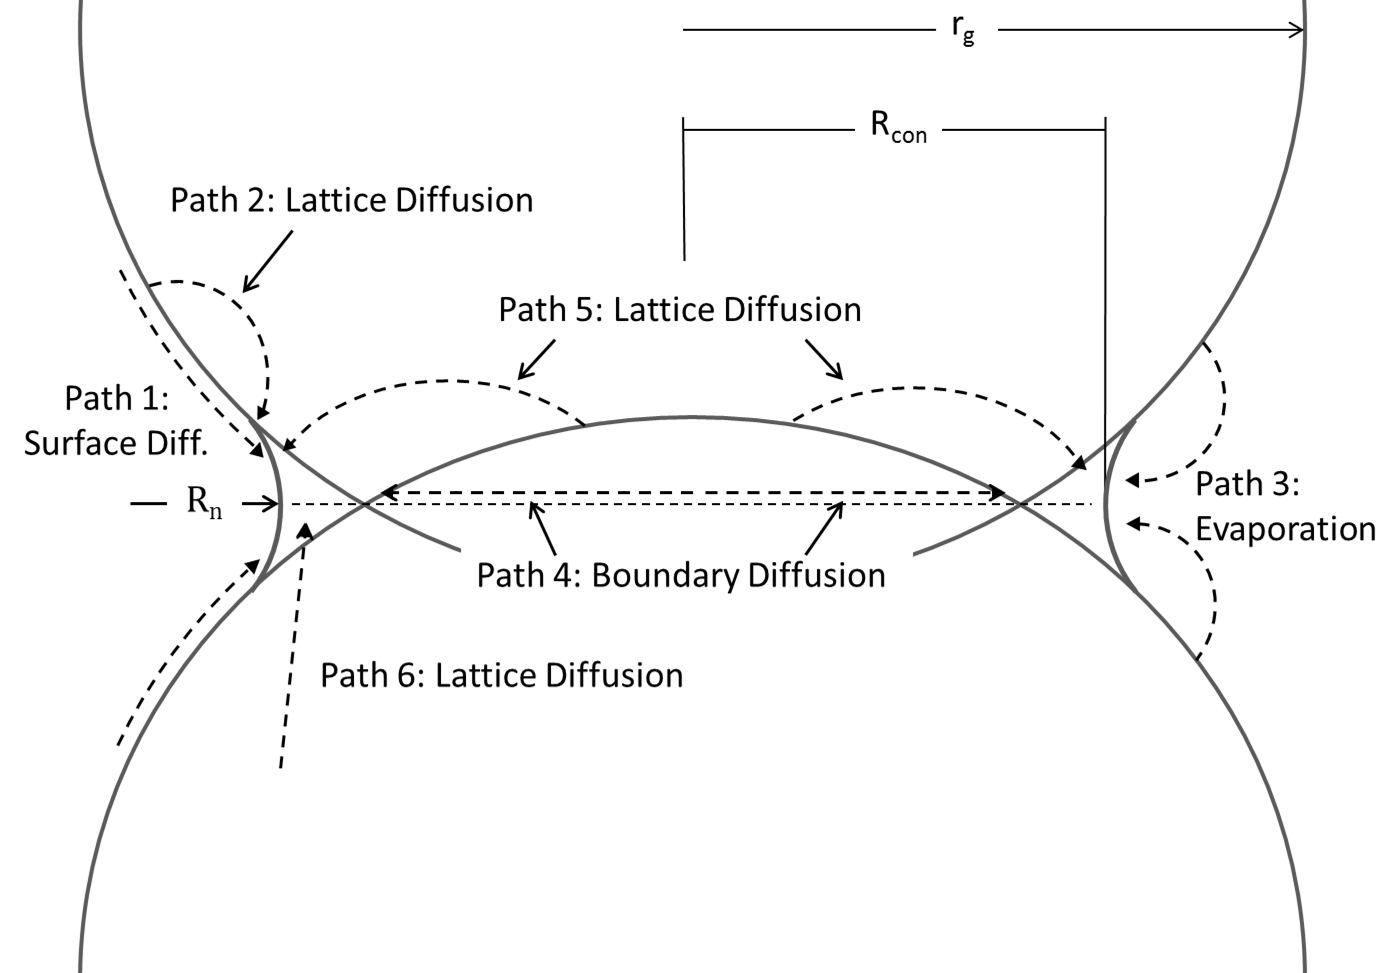
\includegraphics[scale=0.5]{Swinkels1981_DiffMech.png}
	\caption{Pictorial description of the six sintering mechanisms defined by Swinkels and Ashby (1981) who estimated that the defining equations for the various mechanisms (defined below) were accurate to within a factor of 2.}
	\label{fig:diffmech}
	\end{figure}
	
	\begin{itemize}
	\item Non-densifying Mechanism
		\begin{enumerate}
		\item Surface diffusion from a surface source \\
	$\dot{V_{1}} = \frac{3 \pi R_{con} \delta_{s} D_{s}\gamma_{s} \Omega (K_{3}-K_{2})}{d_{2}k_{B}T}$
		\item Lattice diffusion from a surface source \\
	$\dot{V_{2}} = \frac{3 \pi R_{con} D_{v}\gamma_{s} \Omega (K_{3}-K_{m})}{k_{B}T}$
		\item Vapour transport from a surface source \\
	$\dot{V_{3}} = 2 \pi R_{con} R_{n} \theta P_{v} \frac{\gamma_{s} \Omega}{k_{B}T}\left[ \frac{\Omega}{2 \pi \rho_{b} k_{B}T} \right]^{1/2} (K_{3}-K_{m})$
		\end{enumerate}
	\item Densifying Mechanism
		\begin{enumerate}
		\setcounter{enumi}{3}
		\item Grain boundary diffusion from a bourdary source \\
	$\dot{V_{4}} = \frac{16\pi \delta_{b} D_{b}\gamma_{s}\Omega}{R_{con}k_{b}T}\left(1-\frac{K_{1}R_{con}}{2}\right)$
		\item Lattice diffusion from a boundary source \\
	$\dot{V_{5}} = \frac{32\pi R_{n} \theta D_{v}\gamma_{s}\Omega}{R_{con}k_{b}T}\left(1-\frac{K_{m}R_{con}}{2}\right)$
		\item Lattice diffusion from dislocation sources \\
	$\dot{V_{6}} = \frac{8\pi R_{con}^{2} R_{n} \theta N D_{v}\gamma_{s}\Omega}{9 k_{b}T}\left(-K_{m}-\frac{3 \tau R_{con}}{2 \gamma_{s} r_{g}}\right)$
		\end{enumerate}
	\end{itemize}
	
	where
	
	\begin{itemize}
	\item	$R_{n}$ = neck curvature radius ($cm$) 
	\item	$K_{1-3}$ = "curvatures" defined for specific geometry ($cm^{-1}$) 
	\item	$K_{m}^{2}$ = $K_{1}K_{2}$ 
	\item	$\delta_{s}$ = effective surface thickness ($cm$) 
	\item	$\delta_{b}$ = effective grain boundary thicknesss ($cm$) 
	\item	$D_{s}$ = surface diffusion coefficient ($cm^{2}/s$) 
	\item	$D_{v}$ = lattice diffusion coefficient ($cm^{2}/s$) 
	\item	$D_{b}$ = grain boundary diffusion coefficient ($cm^{2}/s$) 
	\item	$\gamma_{s}$ = surface free energy ($J/m^{2}$) 
	\item	$\gamma_{b}$ = grain boundary free energy ($J/cm^{2}$) 
	\item	$\rho_{b}$ = bulk density ($g/cm^{3}$) 
	\item	$\Omega$ = molar volume ($cm^{3}$) 
	\item	$\mu$ = molar mass ($g$)  
	\item	$\tau$ = shear modulus ($dyne/cm^{2}$) 
	\item	$N$ = dislocation density ($cm^{-3}$) 
	\end{itemize}
	
	The rate of growth of the neck region between grains is thus a function of the energy deposition rate and by extension by the various diffusion and desorption rates of atoms and molecules into the contact region.
	
	\begin{equation}
	\frac{dR_{con}}{dt} = \dot{R_{con}} = \frac{\sum_{i=1}^{6} \dot{V_{i}}}{2\pi R_{con} \theta \rho}
	\end{equation}
	
	Kossacki et al (1994) gave an estimate for the neck growth rate due to vapor transport driven by thermal desorption from the grain surface. Vapor desorption and redeposition is likely the dominant sintering mechanism at $\sim$200K, though it may not be relevant at Mimas surface temperatures.
	
	\begin{equation}
	\dot{V_{3}} = \frac{\Omega^{2}\gamma p A_{n}}{(2\pi\mu RT)^{1/2}RT} \left( \frac{2}{r_{g}} + \frac{1}{\rho_{b}} - \frac{1}{R_{con}} \right)
	\end{equation}
	
	The pressure $p$ due to sublimation of molecules from the pore surfaces can be calculated using the Clausius-Clapeyron equation given earlier (Eq.\ref{eq:CCpres}), and the the neck surface area is given by
	
	\begin{equation}
	A_{n} = 4\pi\rho \left[ (R_{con} + \rho)arcsin\left(\frac{r_{a}}{\rho}\right) - r_{a} \right]
	\end{equation}
	
	where $r_{a}$ and $\rho$ are defined by
	
	\begin{equation}
	\rho = \frac{R_{con}^{2}}{2(r_{g}-R_{con})}
	\end{equation}
	
	and
	
	\begin{equation}
	 r_{a} = \frac{r_{g}\rho}{r_{g}+\rho}
	\end{equation}
	
	\emph{I think the goal here should be to relate the warming of the grain due to a electron ineratction with the regolith to a average desorption rate. I am imagining this as the number of electeron interactions per surface area per time, multiplied by an average number of desorbed molecules per event to give number of desorbed molecules per area per time.}
	
	%REJ - ! One thing you can show quickly  is--I think Swinkel and Ashby probably do steady state things. Therefore you can divide an estimate of the energy flux from Paranicas by the penetration depth Rp to get an average heating rate per unit time which I think the effect will be pretty small--rather the time scales very large  -this is not a large amount of heat--compared to what the sun deposits--or maybe simply point that out. Therefore our idea is, it is the individual excitations causing the sintering. Each excitations e can think of as producing a small heat spike randomly in the grain and causing surface molecules to be mobile.  First presume the heat transients in the grain decay rapidly compared to the time the next electron hits that grain---I am sure that is a good assumption. Therefore we would like to use an energy deposition profile--first to determine the grain heating - dE/dz in to the material at each depth z -- assuming all the energy deposited stays in the grain--that would be an upper limit--then the energy density deposited heats the grain to a T determine by $(\rho C T) \sim (dE/z)/pi r^{2}, assuming a fresh surface--no irradiation-- that T decays due to thermal conductivity in the out side region and one can estimate the amount of sublimation. Think about this and comment!

%REJ - 
\begin{Comment}
On using your energy deposition results:

The W value for H2O is ~ 27eV--this means that for an amount of electronic energy deposited, Ee, in an H2O gas, the average number of ionizations is ~Ee/W. We, of course, are interested in ice-- and the rule of thumb is
W ~ 2.5 x electron-hole pair production in a solid --which is somewhat smaller than the gas-phase ionization energy. So I think using a W ~ 20eV would give a rough estimate until I find better estimates--so use this for the time being.

Now for the production of defects on the ice-- the concepts is similar. The average energy for producing a vacant is Ev ~ c U where U is the binding energy per molecule of the solid. I seem to remember, but have to look it up, c~ 5, so Ev ~ 5  U (check this). And for ice U ~ 0.5eV  so that Ev ~ 2.5 eV

Similar to the above -- the deposited energy required on average to produce a vacancy is ~ 2.5 x Ev. These are not well measured in ice but are in silicon and other materials -- If correct, then the number of vacancies produced is  ~ Ee / 6eV.

Of course an individual vacancy does not efficiently scatter the near UV light measured in the UV filter discussed in Schenk et al. The scale is wrong --- Vacancy diameter  is  ~ 10^-3 um whereas the near UV wave length is  ~ 0.3 um. Vacancies of course diffuse under thermal cycling forming larger voids with O2 H2O2 or other radiation products inside--so the light scattering estimate will be a little crude.

There is also another approach to the other aspect--your estimates of contact areas. Ujwall wrote a number of papers on ice compaction ( you cna see in my proposal-- I mention them and he probably has a web site). They were interested in interstellar grains. Compaction is similar to an increase in the contact area. Although mostly they used heavier ions --I think he also did compaction with KeV protons. Since the nuclear stopping is relatively small compared to the electronic stopping we could use that for a rough proxy for the electronic energy deposited by electrons, although we have to be a little careful that the nuclear stopping is not doing the damage.

That is--larger surface areas in contact means slightly smaller void space can change in the shape of the grains--as in the last model (figure) you discuss in your report where they have a certain amount of material 'cut out'
of the spherical grains at the contact point. Therefore a good exercise to think about now that you have the change in contact area is -- imagine as requiring a change in shape at the contact point related to your area increase --as in that figure shows -- see if you can then think about whether or not you can turn the compaction into a change in contact using that model.
\end{comment}
	
	The electronic structure of ice at the interface of large porous cavities in amorphous ice may resemble that of the free surface interface, and therefore it might be expected that ESD processes would occur there with similar mechanisms. The total ESD neutral product yields are generally much higher from amorphous ice than from crystalline. This is attributed to increased defect density and an increase in excitation localization due to disruption of long range order in the matrix [Sieger and Orlando, Surf. Sci. 451(2000) 97].

\section{Regolith gardening rate}


\newpage

\section{Appendiux 1: Review of measured Parameters}
\label{sec:measured}

\subsection{Thermal Inertia (I) - Howett et al. (2011)}
\label{sec:inertia}

	\begin{equation}
	I = \sqrt{kc\rho} \: [\frac{J}{m^{2} K^{1} s^{1/2}}]
	\end{equation}

	\hspace{1cm}
	Where
	\begin{itemize}[leftmargin=3cm]
	\item k = thermal conductivity $[\frac{J}{m \cdot s \cdot K}]$
	\item c = specific heat $[\frac{J}{g \cdot K}]$
	\item $\rho$ = density $[\frac{g}{m^{3}}]$
	\end{itemize}

	The thermal inertial measured by Cassini CIRS was reported by Howett et al. (2011, 2012)
	\begin{itemize}
		\item For Mimas:
		\begin{itemize}
			\item Within anomaly: \fbox{$66 \pm 23  [\frac{J}{m^{2} K^{1} s^{1/2}}]$}
			\item Outside anomaly: \fbox{$< 16  [\frac{J}{m^{2} K^{1} s^{1/2}}]$}
		\end{itemize}
		\item For Tethys:
		\begin{itemize}
			\item Within anomaly: \fbox{$25 \pm 3$ MKS}
			\item Anomaly boundary: \fbox{$11 \pm 1$ MKS}
			\item Outside anomaly: \fbox{$5 \pm 1$ MKS}
		\end{itemize}
	\end{itemize}
		
	\emph{Depth of penetration for CIRS wavelength light?}
	
\subsection{Temperature ranges - Howett et al. (2011)}
\label{sec:temperature}

	Estimated Mimas daytime temperatures: 40-95 K
	
\subsection{Average Particle Size}
\label{sec:size}

%In the UV, Mimas is nearly as bright as Enceladus. Tethys is surprisingly dark in the UV.
%Modeling (Hamilton and Burns, 1994) showed that e-ring grains at the orbit of Mimas (inside the 3.95 R$_{s}$ orbit of Enceladus) are expected to coat the trailing hemisphere of the moon, while at Tethys and other satellites exterior to Enceladus, the e-ring grains impact primarily on the leading hemispheres. 
	
Particle size (diameter) measured using the Cassini observations and, assuming pure water ice regoliths, comparing the water ice absorption band depths at 2.0$\mu m$ and 1.52$\mu m$ to a model correlating absorption depth to grain size developed by Clark and Lucey (1984).

	\begin{itemize}
	\item Mimas: (Hendrix et al, 2012)
	\begin{itemize}
		\item Leading hemisphere: 20-80 $\mu$m
		\item Trailing hemisphere: 10-50 $\mu$m
		\item Herschel crater: 50-100 $\mu$m
	\end{itemize}

	\item Tethys: (Fillachione et al, 2012)
	\begin{itemize}
		\item Average: 30 $\mu$m
		\item Pure H$_{2}$O ice: 22 - 880 $\mu$m
		\item Mixed grains: 69 $\mu$m
	\end{itemize}

	\item Dione (assuming pure water ice): (Newman et al, 2009)
	\begin{itemize}
		\item Whispy region: 6-28 $\mu$m
		\item Dark area: 1-8 $\mu$m
		\item Background: 7-28 $\mu$m
	\end{itemize}
	\end{itemize}

\subsection{Porosity}
\label{sec:porosity}

	The density of a porous medium is given by $\rho_{\phi} = \rho_{0}*(1-\phi)$ where $\rho_{0}$ is the density of the bulk substance. 

	\begin{itemize}
	\item For Enceladus - Verbischer et al (2005): $~50-70\%$
	\item For Tethy's - Caravano et al. (2007): $>90\%$ 
	\item Model parameter (ansatz) Leliwa-Kopystynski (2000): $~50\%$
	\end{itemize}
	
\subsection{Density}
	Density of 50\% porous water ice = 0.934*(1-0.5) = 0.467 g/cm$^{3}$
	
\section{List of Variables}
$\phi$ = porosity
$\chi$ = cementation volume fraction
$\nu_{s}$ = solid volume fraction

\section{Tabulated Literature Parameters}
\label{sec:tabulated}
	
\subsection{Thermal Conductivity}
\label{sec:tconductivity}
	
	Low temperature thermal conductivity
	
	\begin{itemize}
	\item Water Ice
		\begin{itemize}
		\item Ellsworty and Schubert (1983): $k_{ice} = \frac{488.12}{T} +0.4685 \: [\frac{J}{m s K}]$
		\item Haruyama et al (1993) via. Sirono and Yamamoto (1997):
			\begin{itemize}
			\item Amorphous: $k_{H_{2}O, a} = k_{ao} \times T$ where $k_{ao} = 7.1x10^{-3} \: [\frac{erg}{cm s K}]$
			\item Crystalline: $k_{H_{2}O, c} = k_{co}/T$ where $k_{co} = 5.67x10^{7} \: [\frac{erg}{cm s K}]$
			\end{itemize}
		\item Kossacki et al. (1994): $k = \frac{567}{T} \: [\frac{J}{m s K}]$
		\item Klinger (1975): $k_{100 K} = 0.04  \: \frac{J}{m s K}$ (amorphous)
		\\
		then
		\\
		\item Ellsworty and Schubert = 6.57 MKS
		\item Haruyama et al = 7.088 MKS
		\item Kossacki et al = 7.088 MKS
		\end{itemize}
		
%	\item Silicates
%		\begin{itemize}
%		\item Basalt
%			\begin{itemize}
%			\item Clauser (1995) - Bulk: k $\approx 1.5 - 3.5 [ \frac{J}{m \cdot s \cdot K}]$
%			\item Fountain and West (1970) - Crushed (37-62 $\mu m, \rho = 0.9 g/cm^{3}$, T=150K): k $\approx 7\times10^{-4} [\frac{J}{m \cdot s \cdot K}]$
%			\end{itemize}
%		\item Quartz
%			\begin{itemize}
%			\item engineeringtoolbox.com - Bulk: k $\approx 3.0 [\frac{J}{m \cdot s \cdot K}]$
%			\item Smoluchowski (1910) - Crushed (94$\mu$m): k $\approx 3.0 [\frac{J}{m \cdot s \cdot K}]$
%			\end{itemize}
%		\item Pumice
%			\begin{itemize}
%			\item  Hemmings et al. (2009) - Bulk: k $\approx 0.4269 [\frac{J}{m \cdot s \cdot K}]$
%			\item Wechsler and Glaser (1965) - Crushed (44-104 $\mu$m): 
%			\end{itemize}
%		\end{itemize}
	\end{itemize}

\subsection{Specific  and Latent Heat}
\label{sec:sheat}

	Low temperature specific heat:
	
	\begin{itemize}
	\item Ramirez et al. (2012): $c_{100 K} ~ 0.83 [\frac{J}{g K}]$
	\item NBS Monograph 21 (): $c_{100 K} = 0.82 [\frac{J}{g K}]$
	\item Gutierrez et al. (2001): $c_{H_{2}O} = (0.9 + 0.00749 * T) [\frac{J}{g K}]$
		$\rightarrow c_{H_{2}O}(80K) = 1.50 J/g\cdot K$
	\end{itemize}
	
	Latent heat of sublimation:
	
	\begin{itemize}
	\item Gutierrez et al. (2001): $L = 48600 [\frac{J}{mol}]$
	\end{itemize}

\section{Appendix 2: Calculations}

\begin{itemize} 
\item Skin Depth (calculated for Mimas - outside anomaly)
	\begin{equation}
	\begin{split}
	\delta_{out} &= \frac{I_{out}}{\rho_{regolith} c \sqrt{\omega}}  \\
	&= \frac{I_{out}}{(1-\phi)\rho_ {ice} c \sqrt{\omega}} \\
	&= \frac{16[\frac{J}{m^{2} s^{1/2} K}]}{(1-0.5)0.934[\frac{g}{cm^{3}}]0.8[\frac{J}{g \cdot K}]\sqrt{7.7\time10^{-5}[\frac{rad}{s}]}} \\
	\Rightarrow \delta_{out}&= 0.49\: [cm]
	\end{split}
	\end{equation}
	
\item Thermal conductivity determinations
	
\item Number of grains traversed (assume 50um grains)
	\begin{equation}
	\begin{split}
	\text{CSDA ranges: 1 - 10 MeV} &\varpropto 0.4 - 5.0 g/cm^{2} \\
	\text{Total Path Length} S &= \frac{CSDA}{(1-\phi)\cdot\rho_{ice}} \\
	\text{For } \phi &= 0.5 \\
	\Rightarrow S &= 0.85 - 10.6 cm \\
	\text{Number of grains traversed} N &= \frac{2S}{d} \\
	\text{For} d &= 50 \mu m \\
	\Rightarrow N &= 340 - 4240 \\
	\end{split}
	\end{equation}

\item Radiative thermal conductivity
	\begin{equation}
	\begin{split}
	\Rightarrow \epsilon' &= 1 \\
	\Rightarrow \psi &= \frac{1+F}{1-F} \approx 1.087 \\
	\Rightarrow k_{rad} &= 4 (1.087)(5\times10^{-5} m)(5.67\times10^{-8} \frac{J}{m^{2} s K^{4}}(80 K)^{3}) \\
	\Rightarrow k_{rad} &= 6.3\times10^{-6} \frac{J}{m \cdot s \cdot K}
	\end{split}
	\end{equation}

\item Sublimation Heat Transfer
	\begin{equation}
	\begin{split}
	k_{lat} = [ \frac{18 \frac{g}{mol} \times N_{A}}{2 \pi k_{b} (80K)} ]^{1/2} (48600 \frac{J}{mol} & \times N_{A})(0.9 \cdot 50\times10^{-6} m) [ \frac{(3.56\times 10^{12} \frac{N}{m^{2}})(6141.7 K)}{(80 K)^{2}} exp( \frac{-6141.7}{80} ) ] \\
	\Rightarrow k_{lat} &= 1.15\times10^{-26}\frac{J}{m \cdot s \cdot K}
	\end{split}
	\end{equation}

\item Wood 2011 simplification
	\begin{equation}
	\begin{gathered}
	k_{c,max} = k_{ice} \frac{\chi + 1 - \phi}{\chi + 1 + \frac{\phi}{2}} \\
	\Rightarrow k_{eff} = f_{sc} k_{c,max} = f_{sc} k_{ice} \frac{\chi + 1 - \phi}{\chi + 1 + \frac{\phi}{2}} \\
	\\
	\text{assuming   } \chi << \phi  \Rightarrow k_{eff}=2 f_{sc} k_{ice} \frac{1-\phi}{2+\phi}
	\end{gathered}
	\end{equation}
	
\item Wood 2011 contact area and ratio
	\begin{equation}
	\begin{split}
	N_{c} &= 2.02 \left( \frac{1+87.38(1-\phi)^{4}}{1+25.81(1-\phi)^{4}} \left) \\
	&\text{let $\phi$ = 0.5} \\
	N_{c} &= 4.99 \\
	&\text{Then} \\
	f_{sc} &= Y_{sc}N_{c} \left( \frac{N_{c}}{2\sqrt{N_{c}-1}} \frac{R_{con}}{r_{g}} \right)^{Z_{sc}} \\
	&\text{For Z$_{sc}$ = 1, Y$_{sc}$ = 0.09, and r$_{g}$ = 50$\mu$m} \\
	f_{sc} &= 0.01122 R_{con} \text{where R$_{con}$ is in $\mu$m} \\
	&\text{Using Z$_{sc}$ = 2 instead} \\
	f_{sc} &= 0.00028 R_{con} \\
	&\text{Assuming the volume fraction cementation is $<<$ porosity} \\
	k_{eff}=2 f_{sc} k_{ice} \frac{1-\phi}{2+\phi} \\
	&\text{For Mimas, k$_{eff, in} = 0.0113 MKS and k$_{eff, out}$ = .00067 MKS} 
	$\Rightarrow R_{con, in} &= 0.360 \mu m, R_{con,out} = 0.021 \mu m \text{for Z_${sc}$ = 1} \\
	$\Rightarrow R_{con, in} &= 14.4 \mu m, R_{con,out} = 0.854 \mu m \text{for Z_${sc}$ = 2} \\
	&\text{This corresponds to} \\
	\frac{R_{con,in}}{R_{con,out}} = 14.14 \text{for Z$_{sc}$ = 1 and } = 16.86 \text{for Z$_{sc}$ = 2} 
	\end{split} 
	\end{equation}
	
	\begin{Table} \label{tab:Wood2013}
	\caption{Effective grain contact radius and ratio between inside and outside the anomalous regions as calculated using the theory of Wood 2013. Fitting parameters were taken from Wood (2013) and the values used for $k_{ice}$, $r_{g}$, $\phi$ and $k_{eff}$ are given in the text.}
	\centering
		\begin{tabular}[ h, font=small ]{ | c | d | d | d | d | }
		\\ \hline
		\multicolumn{2}{c | }{Mimas} & \multicolumn{2}{ | c |}{Tethys} \\ \hline
		& \multicolumn{1}{c |$Z_{sc} = 1$} & \multicolumn{1}{c |$Z_{sc} = 2$} & \multicolumn{1}{c |$Z_{sc} = 1$} & \multicolumn{1}{c |$Z_{sc} = 2$} \\ \hline
		$R_{con,in}$ & $0.360 \mu m$ & $14.4 \mu m$ & 0.0519 & 0.0021 \\ \hline
		$R_{con,out}$ & $0.021 \mu m$ & $0.854 \mu m$ & 2.077 & 0.083 \\ \hline
		Ratio $\frac{R_{con,in}}{R_{con,out}}$ & \centercell{17.14} & \centercell{16.86} & \centercell{24.95} & \centercell{25.02} \\ \hline
		\end{tabular}
	\end{table}
	
\item Steiner and K\:{o}mle 1991 simplification
	\begin{equation}
	\begin{gathered}
	k_{eff} = (1-\sqrt{1-0.5})(0.5)(6.3\times10^{-6}) + \sqrt{1-0.5} [ H \cdot 7.09+(1-0.5)\frac{1.25+1}{1.25}\frac{(7.09)(6.3\times10^{-6})}{(7.09+6.3\times10^{-6})} ] \\
	\Rightarrow k_{eff} = ( 4.93\times 10^{-6} + 2.24\cdot H )  \frac{J}{m \cdot s \cdot K} \\
	\Rightarrow k_{eff} \approx \sqrt{1-\phi}\cdot H \cdot k_{ice}(T)
	\end{gathered}
	\end{equation}

\item Sirono and Yamamoto 1997 expression variations
	\begin{equation}
	\begin{gathered}
	k_{eff}=k_{ice}\left( \frac{p-p_{c}}{1-p_{c}} \right) \frac{\pi R_{con}^{2}}{gr^{2}} \\
		 =k_{ice}\left( \frac{p-p_{c}}{1-p_{c}} \right) \frac{\pi}{g r^{2}} H^{2} \\
		 = k_{ice}\left( \frac{p-p_{c}}{1-p_{c}} \right) \frac{\pi}{g r^{2}}[ \frac{9 \pi \gamma r^{2} (1-\mu^{2})}{8 E} ]^{2/3}
	\end{gathered}
	\end{equation}
	
\item Sirono and Yamamoto Contact Area
	\begin{equation}
	\begin{gathered}
	S_{in} = \frac{k_{eff, in}}{k_{ice}} \frac{1-p_{c}}{p - p_{c}}\cdot g r_{grain}^{2} \\
	= \frac{0.00113}{7.09} \frac{1-1/3}{0.955-1/3} \cdot (4)(50 \mu m)^2 \\
	\Rightarrow S_{in} = 1.71\times 10^{-11} m^{2} \\
	\Rightarrow S_{out} = 1.00\times 10^{-12} m^{2}
	\end{gathered}
	\end{equation}
	
\item Grain radius simplification
	\begin{equation}
	\begin{split}
	\frac{H_{in}}{H_{out}} &= \frac{k_{in}}{k_{out}} = \frac{r_{in}^{2/3} \xi(r_{in}, \phi)}{r_{out}^{2/3} \xi(r_{out}, \phi)} \\
	\Rightarrow \frac{H_{in}}{H_{out}} &= \frac{r_{in}^{2/3} \frac{N_{A}(r_{in})}{N_{L}(r_{in})}}{r_{out}^{2/3} \frac{N_{A}(r_{out})}{N_{L}(r_{out})}} \\
	& \text{where }\: N_{A}\varpropto \frac{1}{r^{2}} \: \text{and} \: N_{L}\varpropto \frac{1}{r} \\
	\Rightarrow \frac{r_{in}}{r_{out}} &= (\frac{H_{out}}{H_{in}})^{3}
	\end{split}
	\end{equation}

\item Gundlach and Blum 2012 extension of Hertz analysis to aggregates
	 This thermal conductivity equation can be modified to describe a porous regolith layer composed not simply of spherical grains, but of grain aggregates which themsleves are composed of ice grains and which have their own unique materials parameters such as volume filling factor, Poisson's ratio, Young's modulus, and specific surface energy. Taking the volume filling factor (V$_{F}=1-\phi$) of the layer to be the product of the volume filling factors of the aggregates themselves and the volume filling factor of the aggregate structure ($V_{F, layer} = V_{F, agg} V_{F, struc}$), we can write the effective thermal conductivity of the layer as:
	 
	 \begin{equation}
	 \begin{split}
	 k_{layer}(r_{0}, R, T, V_{F, struc}, V_{F, agg}) = \\
	 k_{agg}(r_{0}, T, V_{F, agg}) [\frac{9}{4} \frac{1 - \mu_{agg}^{2}}{E_{agg}(T)}  \pi \gamma_{agg}(T) r^{2}]^{1/3} \xi(R, V_{F, struc})
	 \end{split}
	 \end{equation}
	 
	 where $R$, $E_{agg}$, and $\mu_{agg}$ are the radius, Young's modulus, and Poisson's ratio of the aggregates, respectively. Taking $r_{0}$ to be the grain radius (the size of the grains that make up the aggregate), the specific surface energy of the aggregates can be calculated by:
	 
	 \begin{equation}
	 \gamma_{agg}(T) = V_{F, agg} \gamma_{ice}^{5/3}(T)[\frac{9 \pi (1-\mu_{agg}^{2})}{r_{0} E_{ice}(T)}]^(2/3)
	 \end{equation}
	 
	 The thermal conductivity of the aggregates can be calculated as before:
	 
	 \begin{equation}
	 k_{eff}(r_{0}, T, V_{F, agg} = k_{ice}(T) [\frac{9 (1-\mu_{ice}^{2})}{4 E_{ice}(T)}\pi \gamma_{ice}(T) r_{0}^{2} ]^{1/3}\xi(r_{0}, V_{F, agg})
	 \end{equation}

\end{itemize}

\section{Appendix 3: Summary of thermal conductivity models}
 Conductivity through grains is limited by the contact area between adjacent grains. Several models are discussed in the following and summarized here for ease of comparison.
	
	\begin{itemize}
	\item Wood (2013)
		\begin{equation}
		k_{eff}  = f_{sc} k_{ice} \frac{\chi + 1 - \phi}{\chi + 1 + \frac{\phi}{2}} \\
		\end{equation}
		
		where $\chi$ is the volume fraction of cement. Taking $\phi = 0.5$ and assuming $\chi << \phi$ this equation simplifies to $k_{eff} \approx \frac{2}{5} f_{sc} k_{ice}$.  The solid continuity factor $f_{sc}$ is a measure of the efficiency of heat transfer through contacts between adjacent grains and is dependent on geometrical packing and contact area, determined by Hertzian analysis and cohesive surface forces (JKR theory), between adjacent grains.
		
		\begin{equation}
		f_{sc} = Y_{sc}N_{c} \left( \frac{N_{c}}{2\sqrt{N_{c}-1}} \frac{R_{con}}{r_{g}} \right)^{Z_{sc}}
		\end{equation}
	
	Here, R$_{con}$ is the radius of the contact area, r$_{g}$ is the particle radius, N$_{c}$ is the coordination number, Z$_{sc}$ depends on the ratio of solid to void thermal conductivities and, in the case considered here of low temperature and pressure, can be taken to be 1, and the $Y_{sc}$ factor is a fit to experimental data. %The coordination number can be calculated exactly for regular packings of monodisperse spheres, with N$_{c}$ = 6 for simple cubic packing, and for small, cohesive, nearly spherical particles Yang et al (2000) gave a functional relationship between coordination number and porosity which closely matches measured and modeled random packings, especially at porosities $\ge$40\%. 
	
%	\begin{equation}
%	N_{c} = 2.02 \left( \frac{1+87.38(1-\phi)^{4}}{1+25.81(1-\phi)^{4}} \right)
%	\end{equation}
		
%	\item  Piqueuz and Christensen (2009b) \\
%		P and Q did not give explicit equations to calculate the thermal conductivity, but provided several larger plots that traced how the thermal conductivity varied with \% cementation, grain size, gas pressure etc. However, their focus was on ~atm pressure environments, and the model failed for very small grain contact areas (low thermal conductivities), and thus is was determined this model was unfit to explain the regolith at Mimas.

	\item Steiner and K\"{o}mle (1991)
		\begin{equation}
		 k_{eff} = \sqrt{1-\phi}\cdot H \cdot k_{ice}(T)
		\end{equation}
		
	Where H is the Hertz factor which determines the contact area between touching grains. Taking $\phi = 0.5$, we can simplify this equation to $ k_{eff} \approx 0.71 H k_{ice}$. The $\sqrt{1-\phi}$ factor of the Steiner and K\"omle model is the only term used to account for the structure of the material.

	\item Gundlach and Blum (2010)
	The Gundlach and Blum model was developed using a mathematical analysis by Chan and Tien (1973) for regularly packed spheres whose contact area is described by Hertzian analysis and where the cohesive forces between spheres are described by JKR theory.
	
		\begin{equation}
		k_{eff} = k_{ice} H \frac{1}{0.531 S(\phi)} \frac{N_{A}}{N_{L}}
		\end{equation}
		
	The factors S$_{\phi}$, N$_{A}$, and N$_{L}$ depend on the specific packing arrangement and can be computed explicitly for regular packing arrangements and H is the Hertz factor. 
	
		\begin{equation}
		 H = [\frac{9}{4} \frac{1-\nu^{2}}{E} \pi \gamma r^{2} ]^{1/3}
		\end{equation}
	
	
	\item Sirono and Yamamoto (1997)
		\begin{equation}
		k_{eff} = k_{ice} \left( \frac{p - p_{c}}{1-p_{c}} \right) \frac{\pi R_{con}^{2}}{g r^{2}}
		\end{equation}
		
		Where R$_{con}$ is the grain contact radius as defined by Hertzian analysis and $p$ is related to the volume filling factor and dependent on the packing. More specifically, $p$ is the probability that a lattice site is occupied with a regolith grain. The Hertz factor used by Sirono and Yamamoto is slightly different than that of Gundlach and Blum:
		
		\begin{equation}
		H = [ \frac{9 \pi \gamma r^{2} (1-\nu^{2})}{8 E} ]^{1/3}
		\end{equation}
		
	\end{itemize}
	
\end{document}
